% Created by tikzDevice version 0.8.1 on 2015-01-17 16:20:40
% !TEX encoding = UTF-8 Unicode
% Calculated string width of -4 as 7.998100
% Calculated character metrics. ascent: 6.611760, descent: 0.000000, width: 8.797910
% Calculated string width of -2 as 7.998100
% Calculated string width of 0 as 4.798860
% Calculated string width of 2 as 4.798860
% Calculated string width of -2.5 as 15.463000
% Calculated string width of 0.0 as 12.263750
% Calculated string width of 2.5 as 12.263750
% Calculated string width of 5.0 as 12.263750
% Calculated string width of -2.5 as 15.463000
% Calculated string width of 0.0 as 12.263750
% Calculated string width of 2.5 as 12.263750
% Calculated string width of 5.0 as 12.263750
% Calculated string width of -2.5 as 15.463000
% Calculated string width of 0.0 as 12.263750
% Calculated string width of 2.5 as 12.263750
% Calculated string width of 5.0 as 12.263750
% Calculated string width of All ICSID Disputes$_{t-1}$ as 94.894090
% Calculated string width of ICSID Treaty-Based$_{t-1}$ as 98.599870
% Calculated string width of Unsettled ICSID$_{t-1}$ as 83.243520
% Calculated string width of ICSID-UNCTAD$_{t-1}$ as 84.923110
% Calculated string width of 1987 as 19.195430
% Calculated string width of 1990 as 19.195430
% Calculated string width of 1993 as 19.195430
% Calculated string width of 1996 as 19.195430
% Calculated string width of 1999 as 19.195430
% Calculated string width of 2002 as 19.195430
% Calculated string width of 2005 as 19.195430
% Calculated string width of 2008 as 19.195430
% Calculated string width of 2011 as 19.195430
% Calculated string width of 1987 as 19.195430
% Calculated string width of 1990 as 19.195430
% Calculated string width of 1993 as 19.195430
% Calculated string width of 1996 as 19.195430
% Calculated string width of 1999 as 19.195430
% Calculated string width of 2002 as 19.195430
% Calculated string width of 2005 as 19.195430
% Calculated string width of 2008 as 19.195430
% Calculated string width of 2011 as 19.195430
% Calculated character metrics. ascent: 8.264620, descent: 0.000000, width: 10.997280
% Drawing Rectangle from x0 = 0.000000, y0 = 0.000000 to x1 = 578.160000, y1 = 433.620000
% Beginning new tikzpicture 'page'
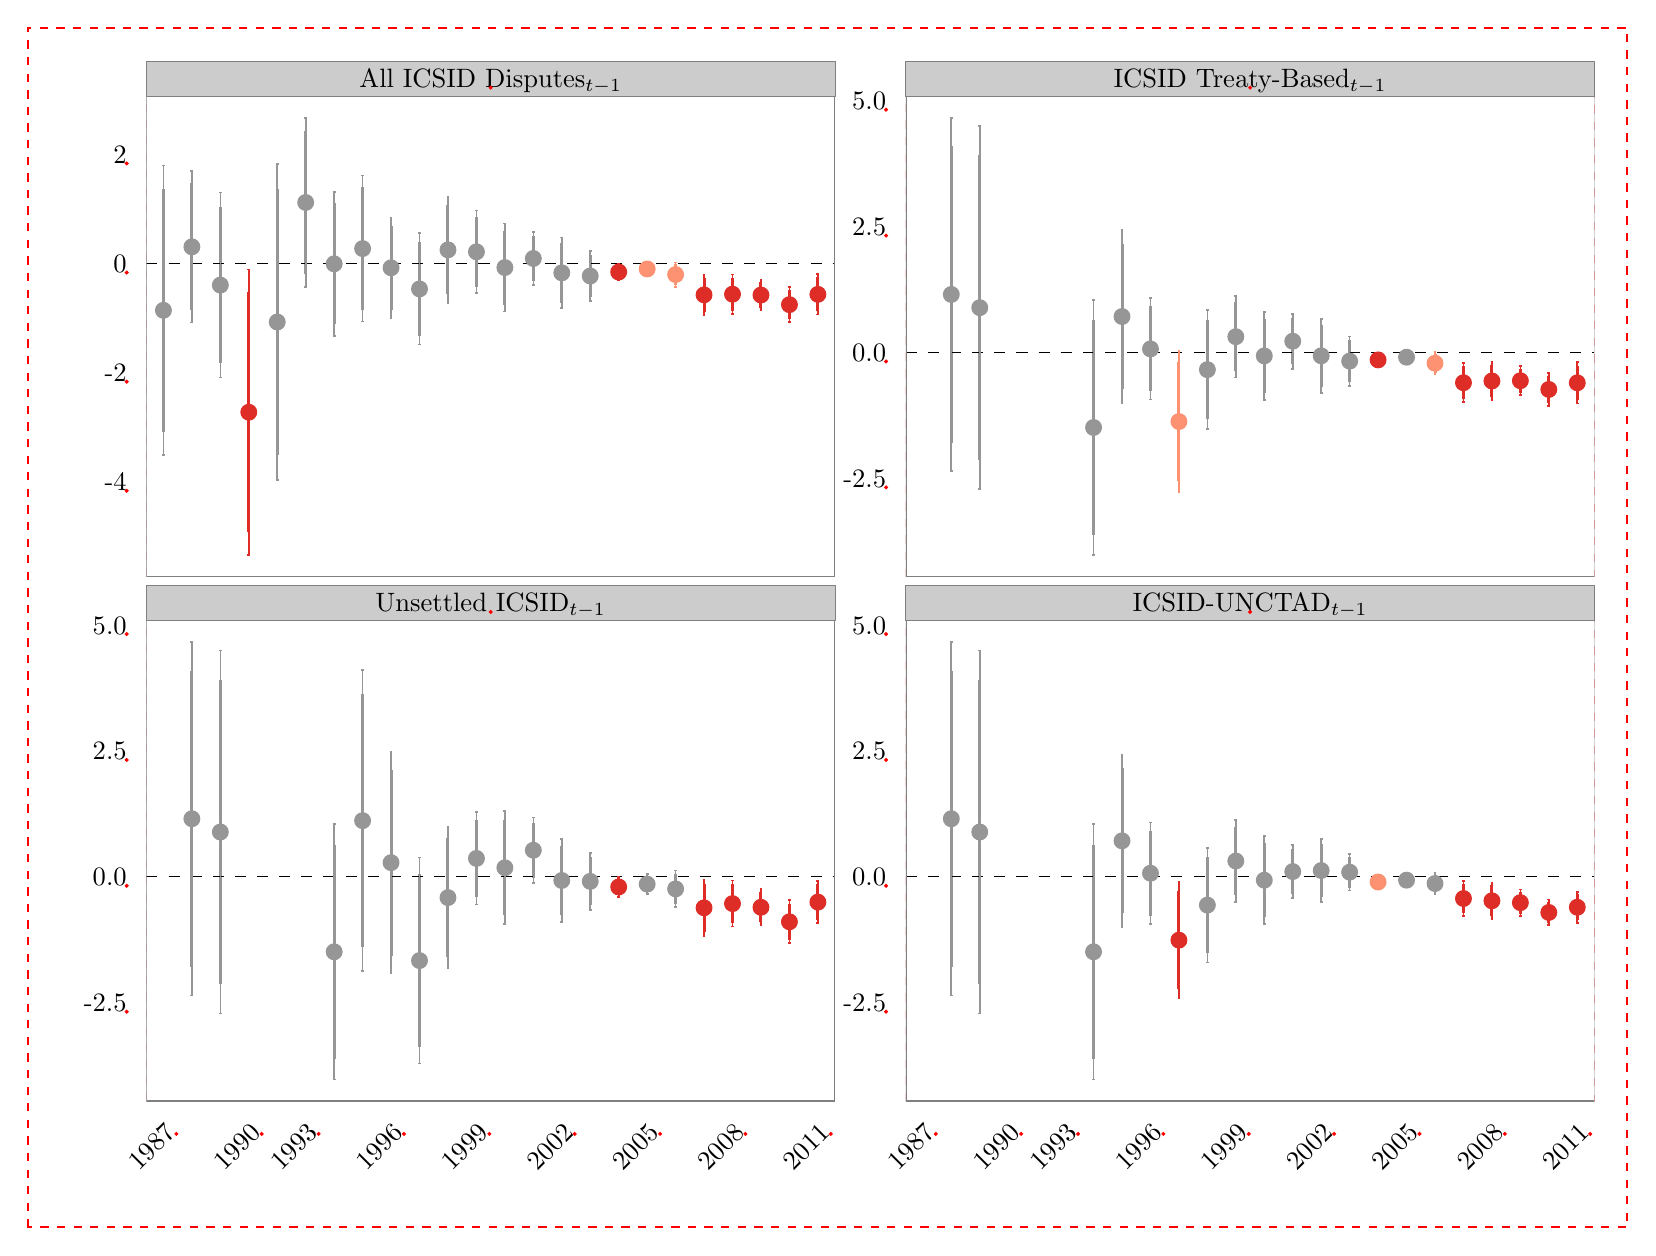
\begin{tikzpicture}[x=1pt,y=1pt]
\definecolor{fillColor}{RGB}{255,255,255}
\path[use as bounding box,fill=fillColor,fill opacity=0.00] (0,0) rectangle (578.16,433.62);
\begin{scope}
\path[clip] (  0.00,  0.00) rectangle (578.16,433.62);
\path[draw=red,very thick,dashed] (  0.00,  0.00) rectangle (578.16,433.62);
\definecolor{drawColor}{RGB}{255,255,255}
\definecolor{fillColor}{RGB}{255,255,255}

\path[draw=drawColor,line width= 0.6pt,line join=round,line cap=round,fill=fillColor] (  0.00,  0.00) rectangle (578.16,433.62);
\end{scope}
% Drawing Rectangle from x0 = 42.885809, y0 = 235.128749 to x1 = 291.706685, y1 = 408.940740
\begin{scope}
\path[clip] ( 42.89,235.13) rectangle (291.71,408.94);
\path[draw=red,very thick,dashed] ( 42.89,235.13) rectangle (291.71,408.94);
\definecolor{fillColor}{RGB}{255,255,255}

\path[fill=fillColor] ( 42.89,235.13) rectangle (291.71,408.94);
% Drawing line from x1 =    49.0549, y1 =   279.1651 to x2 =    49.0549, y2 =   383.7881
\definecolor{drawColor}{RGB}{150,150,150}

\path[draw=drawColor,draw opacity=0.30,line width= 0.3pt,line join=round] ( 49.05,279.17) -- ( 49.05,383.79);
% Drawing line from x1 =    59.3368, y1 =   327.0574 to x2 =    59.3368, y2 =   381.8013

\path[draw=drawColor,draw opacity=0.30,line width= 0.3pt,line join=round] ( 59.34,327.06) -- ( 59.34,381.80);
% Drawing line from x1 =    69.6186, y1 =   307.1779 to x2 =    69.6186, y2 =   374.0232

\path[draw=drawColor,draw opacity=0.30,line width= 0.3pt,line join=round] ( 69.62,307.18) -- ( 69.62,374.02);
% Drawing line from x1 =    79.9005, y1 =   243.0293 to x2 =    79.9005, y2 =   346.2833
\definecolor{drawColor}{RGB}{222,45,38}

\path[draw=drawColor,draw opacity=0.30,line width= 0.3pt,line join=round] ( 79.90,243.03) -- ( 79.90,346.28);
% Drawing line from x1 =    90.1823, y1 =   270.1189 to x2 =    90.1823, y2 =   384.3897
\definecolor{drawColor}{RGB}{150,150,150}

\path[draw=drawColor,draw opacity=0.30,line width= 0.3pt,line join=round] ( 90.18,270.12) -- ( 90.18,384.39);
% Drawing line from x1 =   100.4642, y1 =   339.8667 to x2 =   100.4642, y2 =   401.0402

\path[draw=drawColor,draw opacity=0.30,line width= 0.3pt,line join=round] (100.46,339.87) -- (100.46,401.04);
% Drawing line from x1 =   110.7460, y1 =   322.3010 to x2 =   110.7460, y2 =   374.2680

\path[draw=drawColor,draw opacity=0.30,line width= 0.3pt,line join=round] (110.75,322.30) -- (110.75,374.27);
% Drawing line from x1 =   121.0279, y1 =   327.3990 to x2 =   121.0279, y2 =   380.1732

\path[draw=drawColor,draw opacity=0.30,line width= 0.3pt,line join=round] (121.03,327.40) -- (121.03,380.17);
% Drawing line from x1 =   131.3098, y1 =   328.7575 to x2 =   131.3098, y2 =   364.9378

\path[draw=drawColor,draw opacity=0.30,line width= 0.3pt,line join=round] (131.31,328.76) -- (131.31,364.94);
% Drawing line from x1 =   141.5916, y1 =   319.0701 to x2 =   141.5916, y2 =   359.3517

\path[draw=drawColor,draw opacity=0.30,line width= 0.3pt,line join=round] (141.59,319.07) -- (141.59,359.35);
% Drawing line from x1 =   151.8735, y1 =   334.1507 to x2 =   151.8735, y2 =   372.5148

\path[draw=drawColor,draw opacity=0.30,line width= 0.3pt,line join=round] (151.87,334.15) -- (151.87,372.51);
% Drawing line from x1 =   162.1553, y1 =   337.6665 to x2 =   162.1553, y2 =   367.5738

\path[draw=drawColor,draw opacity=0.30,line width= 0.3pt,line join=round] (162.16,337.67) -- (162.16,367.57);
% Drawing line from x1 =   172.4372, y1 =   331.0079 to x2 =   172.4372, y2 =   362.8625

\path[draw=drawColor,draw opacity=0.30,line width= 0.3pt,line join=round] (172.44,331.01) -- (172.44,362.86);
% Drawing line from x1 =   182.7190, y1 =   340.5997 to x2 =   182.7190, y2 =   359.8189

\path[draw=drawColor,draw opacity=0.30,line width= 0.3pt,line join=round] (182.72,340.60) -- (182.72,359.82);
% Drawing line from x1 =   193.0009, y1 =   332.1998 to x2 =   193.0009, y2 =   357.8426

\path[draw=drawColor,draw opacity=0.30,line width= 0.3pt,line join=round] (193.00,332.20) -- (193.00,357.84);
% Drawing line from x1 =   203.2827, y1 =   334.7709 to x2 =   203.2827, y2 =   352.9870

\path[draw=drawColor,draw opacity=0.30,line width= 0.3pt,line join=round] (203.28,334.77) -- (203.28,352.99);
% Drawing line from x1 =   213.5646, y1 =   342.5201 to x2 =   213.5646, y2 =   348.1160
\definecolor{drawColor}{RGB}{222,45,38}

\path[draw=drawColor,draw opacity=0.30,line width= 0.3pt,line join=round] (213.56,342.52) -- (213.56,348.12);
% Drawing line from x1 =   223.8464, y1 =   344.0696 to x2 =   223.8464, y2 =   348.7962
\definecolor{drawColor}{RGB}{252,146,114}

\path[draw=drawColor,draw opacity=0.30,line width= 0.3pt,line join=round] (223.85,344.07) -- (223.85,348.80);
% Drawing line from x1 =   234.1283, y1 =   339.9923 to x2 =   234.1283, y2 =   348.8070

\path[draw=drawColor,draw opacity=0.30,line width= 0.3pt,line join=round] (234.13,339.99) -- (234.13,348.81);
% Drawing line from x1 =   244.4102, y1 =   329.6640 to x2 =   244.4102, y2 =   344.4674
\definecolor{drawColor}{RGB}{222,45,38}

\path[draw=drawColor,draw opacity=0.30,line width= 0.3pt,line join=round] (244.41,329.66) -- (244.41,344.47);
% Drawing line from x1 =   254.6920, y1 =   330.1725 to x2 =   254.6920, y2 =   344.4520

\path[draw=drawColor,draw opacity=0.30,line width= 0.3pt,line join=round] (254.69,330.17) -- (254.69,344.45);
% Drawing line from x1 =   264.9739, y1 =   331.3731 to x2 =   264.9739, y2 =   342.6189

\path[draw=drawColor,draw opacity=0.30,line width= 0.3pt,line join=round] (264.97,331.37) -- (264.97,342.62);
% Drawing line from x1 =   275.2557, y1 =   327.2241 to x2 =   275.2557, y2 =   339.8410

\path[draw=drawColor,draw opacity=0.30,line width= 0.3pt,line join=round] (275.26,327.22) -- (275.26,339.84);
% Drawing line from x1 =   285.5376, y1 =   329.9668 to x2 =   285.5376, y2 =   344.5495

\path[draw=drawColor,draw opacity=0.30,line width= 0.3pt,line join=round] (285.54,329.97) -- (285.54,344.55);
% Drawing line from x1 =    49.0549, y1 =   287.5754 to x2 =    49.0549, y2 =   375.3778
\definecolor{drawColor}{gray}{0.59}

\path[draw=drawColor,line width= 1.1pt,line join=round] ( 49.05,287.58) -- ( 49.05,375.38);
% Drawing line from x1 =    59.3368, y1 =   331.4581 to x2 =    59.3368, y2 =   377.4006

\path[draw=drawColor,line width= 1.1pt,line join=round] ( 59.34,331.46) -- ( 59.34,377.40);
% Drawing line from x1 =    69.6186, y1 =   312.5514 to x2 =    69.6186, y2 =   368.6497

\path[draw=drawColor,line width= 1.1pt,line join=round] ( 69.62,312.55) -- ( 69.62,368.65);
% Drawing line from x1 =    79.9005, y1 =   251.3295 to x2 =    79.9005, y2 =   337.9830
\definecolor{drawColor}{RGB}{222,45,38}

\path[draw=drawColor,line width= 1.1pt,line join=round] ( 79.90,251.33) -- ( 79.90,337.98);
% Drawing line from x1 =    90.1823, y1 =   279.3048 to x2 =    90.1823, y2 =   375.2039
\definecolor{drawColor}{gray}{0.59}

\path[draw=drawColor,line width= 1.1pt,line join=round] ( 90.18,279.30) -- ( 90.18,375.20);
% Drawing line from x1 =   100.4642, y1 =   344.7843 to x2 =   100.4642, y2 =   396.1227

\path[draw=drawColor,line width= 1.1pt,line join=round] (100.46,344.78) -- (100.46,396.12);
% Drawing line from x1 =   110.7460, y1 =   326.4784 to x2 =   110.7460, y2 =   370.0906

\path[draw=drawColor,line width= 1.1pt,line join=round] (110.75,326.48) -- (110.75,370.09);
% Drawing line from x1 =   121.0279, y1 =   331.6414 to x2 =   121.0279, y2 =   375.9308

\path[draw=drawColor,line width= 1.1pt,line join=round] (121.03,331.64) -- (121.03,375.93);
% Drawing line from x1 =   131.3098, y1 =   331.6659 to x2 =   131.3098, y2 =   362.0294

\path[draw=drawColor,line width= 1.1pt,line join=round] (131.31,331.67) -- (131.31,362.03);
% Drawing line from x1 =   141.5916, y1 =   322.3082 to x2 =   141.5916, y2 =   356.1136

\path[draw=drawColor,line width= 1.1pt,line join=round] (141.59,322.31) -- (141.59,356.11);
% Drawing line from x1 =   151.8735, y1 =   337.2347 to x2 =   151.8735, y2 =   369.4309

\path[draw=drawColor,line width= 1.1pt,line join=round] (151.87,337.23) -- (151.87,369.43);
% Drawing line from x1 =   162.1553, y1 =   340.0707 to x2 =   162.1553, y2 =   365.1696

\path[draw=drawColor,line width= 1.1pt,line join=round] (162.16,340.07) -- (162.16,365.17);
% Drawing line from x1 =   172.4372, y1 =   333.5686 to x2 =   172.4372, y2 =   360.3018

\path[draw=drawColor,line width= 1.1pt,line join=round] (172.44,333.57) -- (172.44,360.30);
% Drawing line from x1 =   182.7190, y1 =   342.1447 to x2 =   182.7190, y2 =   358.2739

\path[draw=drawColor,line width= 1.1pt,line join=round] (182.72,342.14) -- (182.72,358.27);
% Drawing line from x1 =   193.0009, y1 =   334.2612 to x2 =   193.0009, y2 =   355.7813

\path[draw=drawColor,line width= 1.1pt,line join=round] (193.00,334.26) -- (193.00,355.78);
% Drawing line from x1 =   203.2827, y1 =   336.2353 to x2 =   203.2827, y2 =   351.5227

\path[draw=drawColor,line width= 1.1pt,line join=round] (203.28,336.24) -- (203.28,351.52);
% Drawing line from x1 =   213.5646, y1 =   342.9700 to x2 =   213.5646, y2 =   347.6661
\definecolor{drawColor}{RGB}{222,45,38}

\path[draw=drawColor,line width= 1.1pt,line join=round] (213.56,342.97) -- (213.56,347.67);
% Drawing line from x1 =   223.8464, y1 =   344.4495 to x2 =   223.8464, y2 =   348.4163
\definecolor{drawColor}{RGB}{252,146,114}

\path[draw=drawColor,line width= 1.1pt,line join=round] (223.85,344.45) -- (223.85,348.42);
% Drawing line from x1 =   234.1283, y1 =   340.7009 to x2 =   234.1283, y2 =   348.0984

\path[draw=drawColor,line width= 1.1pt,line join=round] (234.13,340.70) -- (234.13,348.10);
% Drawing line from x1 =   244.4102, y1 =   330.8540 to x2 =   244.4102, y2 =   343.2774
\definecolor{drawColor}{RGB}{222,45,38}

\path[draw=drawColor,line width= 1.1pt,line join=round] (244.41,330.85) -- (244.41,343.28);
% Drawing line from x1 =   254.6920, y1 =   331.3204 to x2 =   254.6920, y2 =   343.3042

\path[draw=drawColor,line width= 1.1pt,line join=round] (254.69,331.32) -- (254.69,343.30);
% Drawing line from x1 =   264.9739, y1 =   332.2771 to x2 =   264.9739, y2 =   341.7148

\path[draw=drawColor,line width= 1.1pt,line join=round] (264.97,332.28) -- (264.97,341.71);
% Drawing line from x1 =   275.2557, y1 =   328.2384 to x2 =   275.2557, y2 =   338.8267

\path[draw=drawColor,line width= 1.1pt,line join=round] (275.26,328.24) -- (275.26,338.83);
% Drawing line from x1 =   285.5376, y1 =   331.1391 to x2 =   285.5376, y2 =   343.3772

\path[draw=drawColor,line width= 1.1pt,line join=round] (285.54,331.14) -- (285.54,343.38);
% Drawing line from x1 =    42.8858, y1 =   348.4353 to x2 =   291.7067, y2 =   348.4353
\definecolor{drawColor}{RGB}{0,0,0}

\path[draw=drawColor,line width= 0.6pt,dash pattern=on 4pt off 4pt ,line join=round] ( 42.89,348.44) -- (291.71,348.44);
% Drawing Circle at x = 49.054922, y = 331.476618, r = 2.845276
\definecolor{drawColor}{gray}{0.59}
\definecolor{fillColor}{gray}{0.59}

\path[draw=drawColor,line width= 0.4pt,line join=round,line cap=round,fill=fillColor] ( 49.05,331.48) circle (  2.85);
% Drawing Circle at x = 59.336776, y = 354.429338, r = 2.845276

\path[draw=drawColor,line width= 0.4pt,line join=round,line cap=round,fill=fillColor] ( 59.34,354.43) circle (  2.85);
% Drawing Circle at x = 69.618630, y = 340.600550, r = 2.845276

\path[draw=drawColor,line width= 0.4pt,line join=round,line cap=round,fill=fillColor] ( 69.62,340.60) circle (  2.85);
% Drawing Circle at x = 79.900485, y = 294.656286, r = 2.845276
\definecolor{drawColor}{RGB}{222,45,38}
\definecolor{fillColor}{RGB}{222,45,38}

\path[draw=drawColor,line width= 0.4pt,line join=round,line cap=round,fill=fillColor] ( 79.90,294.66) circle (  2.85);
% Drawing Circle at x = 90.182339, y = 327.254321, r = 2.845276
\definecolor{drawColor}{gray}{0.59}
\definecolor{fillColor}{gray}{0.59}

\path[draw=drawColor,line width= 0.4pt,line join=round,line cap=round,fill=fillColor] ( 90.18,327.25) circle (  2.85);
% Drawing Circle at x = 100.464194, y = 370.453471, r = 2.845276

\path[draw=drawColor,line width= 0.4pt,line join=round,line cap=round,fill=fillColor] (100.46,370.45) circle (  2.85);
% Drawing Circle at x = 110.746048, y = 348.284507, r = 2.845276

\path[draw=drawColor,line width= 0.4pt,line join=round,line cap=round,fill=fillColor] (110.75,348.28) circle (  2.85);
% Drawing Circle at x = 121.027902, y = 353.786090, r = 2.845276

\path[draw=drawColor,line width= 0.4pt,line join=round,line cap=round,fill=fillColor] (121.03,353.79) circle (  2.85);
% Drawing Circle at x = 131.309757, y = 346.847652, r = 2.845276

\path[draw=drawColor,line width= 0.4pt,line join=round,line cap=round,fill=fillColor] (131.31,346.85) circle (  2.85);
% Drawing Circle at x = 141.591611, y = 339.210883, r = 2.845276

\path[draw=drawColor,line width= 0.4pt,line join=round,line cap=round,fill=fillColor] (141.59,339.21) circle (  2.85);
% Drawing Circle at x = 151.873465, y = 353.332779, r = 2.845276

\path[draw=drawColor,line width= 0.4pt,line join=round,line cap=round,fill=fillColor] (151.87,353.33) circle (  2.85);
% Drawing Circle at x = 162.155320, y = 352.620148, r = 2.845276

\path[draw=drawColor,line width= 0.4pt,line join=round,line cap=round,fill=fillColor] (162.16,352.62) circle (  2.85);
% Drawing Circle at x = 172.437174, y = 346.935216, r = 2.845276

\path[draw=drawColor,line width= 0.4pt,line join=round,line cap=round,fill=fillColor] (172.44,346.94) circle (  2.85);
% Drawing Circle at x = 182.719029, y = 350.209314, r = 2.845276

\path[draw=drawColor,line width= 0.4pt,line join=round,line cap=round,fill=fillColor] (182.72,350.21) circle (  2.85);
% Drawing Circle at x = 193.000883, y = 345.021208, r = 2.845276

\path[draw=drawColor,line width= 0.4pt,line join=round,line cap=round,fill=fillColor] (193.00,345.02) circle (  2.85);
% Drawing Circle at x = 203.282737, y = 343.878962, r = 2.845276

\path[draw=drawColor,line width= 0.4pt,line join=round,line cap=round,fill=fillColor] (203.28,343.88) circle (  2.85);
% Drawing Circle at x = 213.564592, y = 345.318040, r = 2.845276
\definecolor{drawColor}{RGB}{222,45,38}
\definecolor{fillColor}{RGB}{222,45,38}

\path[draw=drawColor,line width= 0.4pt,line join=round,line cap=round,fill=fillColor] (213.56,345.32) circle (  2.85);
% Drawing Circle at x = 223.846446, y = 346.432888, r = 2.845276
\definecolor{drawColor}{RGB}{252,146,114}
\definecolor{fillColor}{RGB}{252,146,114}

\path[draw=drawColor,line width= 0.4pt,line join=round,line cap=round,fill=fillColor] (223.85,346.43) circle (  2.85);
% Drawing Circle at x = 234.128300, y = 344.399652, r = 2.845276

\path[draw=drawColor,line width= 0.4pt,line join=round,line cap=round,fill=fillColor] (234.13,344.40) circle (  2.85);
% Drawing Circle at x = 244.410155, y = 337.065702, r = 2.845276
\definecolor{drawColor}{RGB}{222,45,38}
\definecolor{fillColor}{RGB}{222,45,38}

\path[draw=drawColor,line width= 0.4pt,line join=round,line cap=round,fill=fillColor] (244.41,337.07) circle (  2.85);
% Drawing Circle at x = 254.692009, y = 337.312262, r = 2.845276

\path[draw=drawColor,line width= 0.4pt,line join=round,line cap=round,fill=fillColor] (254.69,337.31) circle (  2.85);
% Drawing Circle at x = 264.973864, y = 336.995970, r = 2.845276

\path[draw=drawColor,line width= 0.4pt,line join=round,line cap=round,fill=fillColor] (264.97,337.00) circle (  2.85);
% Drawing Circle at x = 275.255718, y = 333.532562, r = 2.845276

\path[draw=drawColor,line width= 0.4pt,line join=round,line cap=round,fill=fillColor] (275.26,333.53) circle (  2.85);
% Drawing Circle at x = 285.537572, y = 337.258146, r = 2.845276

\path[draw=drawColor,line width= 0.4pt,line join=round,line cap=round,fill=fillColor] (285.54,337.26) circle (  2.85);
% Starting Polyline
\definecolor{drawColor}{gray}{0.59}

\path[draw=drawColor,line width= 0.6pt,line join=round] ( 48.54,383.79) --
	( 49.57,383.79);
% End Polyline
% Starting Polyline

\path[draw=drawColor,line width= 0.6pt,line join=round] ( 49.05,383.79) --
	( 49.05,279.17);
% End Polyline
% Starting Polyline

\path[draw=drawColor,line width= 0.6pt,line join=round] ( 48.54,279.17) --
	( 49.57,279.17);
% End Polyline
% Starting Polyline

\path[draw=drawColor,line width= 0.6pt,line join=round] ( 58.82,381.80) --
	( 59.85,381.80);
% End Polyline
% Starting Polyline

\path[draw=drawColor,line width= 0.6pt,line join=round] ( 59.34,381.80) --
	( 59.34,327.06);
% End Polyline
% Starting Polyline

\path[draw=drawColor,line width= 0.6pt,line join=round] ( 58.82,327.06) --
	( 59.85,327.06);
% End Polyline
% Starting Polyline

\path[draw=drawColor,line width= 0.6pt,line join=round] ( 69.10,374.02) --
	( 70.13,374.02);
% End Polyline
% Starting Polyline

\path[draw=drawColor,line width= 0.6pt,line join=round] ( 69.62,374.02) --
	( 69.62,307.18);
% End Polyline
% Starting Polyline

\path[draw=drawColor,line width= 0.6pt,line join=round] ( 69.10,307.18) --
	( 70.13,307.18);
% End Polyline
% Starting Polyline
\definecolor{drawColor}{RGB}{222,45,38}

\path[draw=drawColor,line width= 0.6pt,line join=round] ( 79.39,346.28) --
	( 80.41,346.28);
% End Polyline
% Starting Polyline

\path[draw=drawColor,line width= 0.6pt,line join=round] ( 79.90,346.28) --
	( 79.90,243.03);
% End Polyline
% Starting Polyline

\path[draw=drawColor,line width= 0.6pt,line join=round] ( 79.39,243.03) --
	( 80.41,243.03);
% End Polyline
% Starting Polyline
\definecolor{drawColor}{gray}{0.59}

\path[draw=drawColor,line width= 0.6pt,line join=round] ( 89.67,384.39) --
	( 90.70,384.39);
% End Polyline
% Starting Polyline

\path[draw=drawColor,line width= 0.6pt,line join=round] ( 90.18,384.39) --
	( 90.18,270.12);
% End Polyline
% Starting Polyline

\path[draw=drawColor,line width= 0.6pt,line join=round] ( 89.67,270.12) --
	( 90.70,270.12);
% End Polyline
% Starting Polyline

\path[draw=drawColor,line width= 0.6pt,line join=round] ( 99.95,401.04) --
	(100.98,401.04);
% End Polyline
% Starting Polyline

\path[draw=drawColor,line width= 0.6pt,line join=round] (100.46,401.04) --
	(100.46,339.87);
% End Polyline
% Starting Polyline

\path[draw=drawColor,line width= 0.6pt,line join=round] ( 99.95,339.87) --
	(100.98,339.87);
% End Polyline
% Starting Polyline

\path[draw=drawColor,line width= 0.6pt,line join=round] (110.23,374.27) --
	(111.26,374.27);
% End Polyline
% Starting Polyline

\path[draw=drawColor,line width= 0.6pt,line join=round] (110.75,374.27) --
	(110.75,322.30);
% End Polyline
% Starting Polyline

\path[draw=drawColor,line width= 0.6pt,line join=round] (110.23,322.30) --
	(111.26,322.30);
% End Polyline
% Starting Polyline

\path[draw=drawColor,line width= 0.6pt,line join=round] (120.51,380.17) --
	(121.54,380.17);
% End Polyline
% Starting Polyline

\path[draw=drawColor,line width= 0.6pt,line join=round] (121.03,380.17) --
	(121.03,327.40);
% End Polyline
% Starting Polyline

\path[draw=drawColor,line width= 0.6pt,line join=round] (120.51,327.40) --
	(121.54,327.40);
% End Polyline
% Starting Polyline

\path[draw=drawColor,line width= 0.6pt,line join=round] (130.80,364.94) --
	(131.82,364.94);
% End Polyline
% Starting Polyline

\path[draw=drawColor,line width= 0.6pt,line join=round] (131.31,364.94) --
	(131.31,328.76);
% End Polyline
% Starting Polyline

\path[draw=drawColor,line width= 0.6pt,line join=round] (130.80,328.76) --
	(131.82,328.76);
% End Polyline
% Starting Polyline

\path[draw=drawColor,line width= 0.6pt,line join=round] (141.08,359.35) --
	(142.11,359.35);
% End Polyline
% Starting Polyline

\path[draw=drawColor,line width= 0.6pt,line join=round] (141.59,359.35) --
	(141.59,319.07);
% End Polyline
% Starting Polyline

\path[draw=drawColor,line width= 0.6pt,line join=round] (141.08,319.07) --
	(142.11,319.07);
% End Polyline
% Starting Polyline

\path[draw=drawColor,line width= 0.6pt,line join=round] (151.36,372.51) --
	(152.39,372.51);
% End Polyline
% Starting Polyline

\path[draw=drawColor,line width= 0.6pt,line join=round] (151.87,372.51) --
	(151.87,334.15);
% End Polyline
% Starting Polyline

\path[draw=drawColor,line width= 0.6pt,line join=round] (151.36,334.15) --
	(152.39,334.15);
% End Polyline
% Starting Polyline

\path[draw=drawColor,line width= 0.6pt,line join=round] (161.64,367.57) --
	(162.67,367.57);
% End Polyline
% Starting Polyline

\path[draw=drawColor,line width= 0.6pt,line join=round] (162.16,367.57) --
	(162.16,337.67);
% End Polyline
% Starting Polyline

\path[draw=drawColor,line width= 0.6pt,line join=round] (161.64,337.67) --
	(162.67,337.67);
% End Polyline
% Starting Polyline

\path[draw=drawColor,line width= 0.6pt,line join=round] (171.92,362.86) --
	(172.95,362.86);
% End Polyline
% Starting Polyline

\path[draw=drawColor,line width= 0.6pt,line join=round] (172.44,362.86) --
	(172.44,331.01);
% End Polyline
% Starting Polyline

\path[draw=drawColor,line width= 0.6pt,line join=round] (171.92,331.01) --
	(172.95,331.01);
% End Polyline
% Starting Polyline

\path[draw=drawColor,line width= 0.6pt,line join=round] (182.20,359.82) --
	(183.23,359.82);
% End Polyline
% Starting Polyline

\path[draw=drawColor,line width= 0.6pt,line join=round] (182.72,359.82) --
	(182.72,340.60);
% End Polyline
% Starting Polyline

\path[draw=drawColor,line width= 0.6pt,line join=round] (182.20,340.60) --
	(183.23,340.60);
% End Polyline
% Starting Polyline

\path[draw=drawColor,line width= 0.6pt,line join=round] (192.49,357.84) --
	(193.51,357.84);
% End Polyline
% Starting Polyline

\path[draw=drawColor,line width= 0.6pt,line join=round] (193.00,357.84) --
	(193.00,332.20);
% End Polyline
% Starting Polyline

\path[draw=drawColor,line width= 0.6pt,line join=round] (192.49,332.20) --
	(193.51,332.20);
% End Polyline
% Starting Polyline

\path[draw=drawColor,line width= 0.6pt,line join=round] (202.77,352.99) --
	(203.80,352.99);
% End Polyline
% Starting Polyline

\path[draw=drawColor,line width= 0.6pt,line join=round] (203.28,352.99) --
	(203.28,334.77);
% End Polyline
% Starting Polyline

\path[draw=drawColor,line width= 0.6pt,line join=round] (202.77,334.77) --
	(203.80,334.77);
% End Polyline
% Starting Polyline
\definecolor{drawColor}{RGB}{222,45,38}

\path[draw=drawColor,line width= 0.6pt,line join=round] (213.05,348.12) --
	(214.08,348.12);
% End Polyline
% Starting Polyline

\path[draw=drawColor,line width= 0.6pt,line join=round] (213.56,348.12) --
	(213.56,342.52);
% End Polyline
% Starting Polyline

\path[draw=drawColor,line width= 0.6pt,line join=round] (213.05,342.52) --
	(214.08,342.52);
% End Polyline
% Starting Polyline
\definecolor{drawColor}{RGB}{252,146,114}

\path[draw=drawColor,line width= 0.6pt,line join=round] (223.33,348.80) --
	(224.36,348.80);
% End Polyline
% Starting Polyline

\path[draw=drawColor,line width= 0.6pt,line join=round] (223.85,348.80) --
	(223.85,344.07);
% End Polyline
% Starting Polyline

\path[draw=drawColor,line width= 0.6pt,line join=round] (223.33,344.07) --
	(224.36,344.07);
% End Polyline
% Starting Polyline

\path[draw=drawColor,line width= 0.6pt,line join=round] (233.61,348.81) --
	(234.64,348.81);
% End Polyline
% Starting Polyline

\path[draw=drawColor,line width= 0.6pt,line join=round] (234.13,348.81) --
	(234.13,339.99);
% End Polyline
% Starting Polyline

\path[draw=drawColor,line width= 0.6pt,line join=round] (233.61,339.99) --
	(234.64,339.99);
% End Polyline
% Starting Polyline
\definecolor{drawColor}{RGB}{222,45,38}

\path[draw=drawColor,line width= 0.6pt,line join=round] (243.90,344.47) --
	(244.92,344.47);
% End Polyline
% Starting Polyline

\path[draw=drawColor,line width= 0.6pt,line join=round] (244.41,344.47) --
	(244.41,329.66);
% End Polyline
% Starting Polyline

\path[draw=drawColor,line width= 0.6pt,line join=round] (243.90,329.66) --
	(244.92,329.66);
% End Polyline
% Starting Polyline

\path[draw=drawColor,line width= 0.6pt,line join=round] (254.18,344.45) --
	(255.21,344.45);
% End Polyline
% Starting Polyline

\path[draw=drawColor,line width= 0.6pt,line join=round] (254.69,344.45) --
	(254.69,330.17);
% End Polyline
% Starting Polyline

\path[draw=drawColor,line width= 0.6pt,line join=round] (254.18,330.17) --
	(255.21,330.17);
% End Polyline
% Starting Polyline

\path[draw=drawColor,line width= 0.6pt,line join=round] (264.46,342.62) --
	(265.49,342.62);
% End Polyline
% Starting Polyline

\path[draw=drawColor,line width= 0.6pt,line join=round] (264.97,342.62) --
	(264.97,331.37);
% End Polyline
% Starting Polyline

\path[draw=drawColor,line width= 0.6pt,line join=round] (264.46,331.37) --
	(265.49,331.37);
% End Polyline
% Starting Polyline

\path[draw=drawColor,line width= 0.6pt,line join=round] (274.74,339.84) --
	(275.77,339.84);
% End Polyline
% Starting Polyline

\path[draw=drawColor,line width= 0.6pt,line join=round] (275.26,339.84) --
	(275.26,327.22);
% End Polyline
% Starting Polyline

\path[draw=drawColor,line width= 0.6pt,line join=round] (274.74,327.22) --
	(275.77,327.22);
% End Polyline
% Starting Polyline

\path[draw=drawColor,line width= 0.6pt,line join=round] (285.02,344.55) --
	(286.05,344.55);
% End Polyline
% Starting Polyline

\path[draw=drawColor,line width= 0.6pt,line join=round] (285.54,344.55) --
	(285.54,329.97);
% End Polyline
% Starting Polyline

\path[draw=drawColor,line width= 0.6pt,line join=round] (285.02,329.97) --
	(286.05,329.97);
% End Polyline
% Drawing Rectangle from x0 = 42.885809, y0 = 235.128749 to x1 = 291.706685, y1 = 408.940740
\definecolor{drawColor}{gray}{0.50}

\path[draw=drawColor,line width= 0.6pt,line join=round,line cap=round] ( 42.89,235.13) rectangle (291.71,408.94);
\end{scope}
% Drawing Rectangle from x0 = 317.294124, y0 = 235.128749 to x1 = 566.115000, y1 = 408.940740
\begin{scope}
\path[clip] (317.29,235.13) rectangle (566.11,408.94);
\path[draw=red,very thick,dashed] (317.29,235.13) rectangle (566.11,408.94);
\definecolor{fillColor}{RGB}{255,255,255}

\path[fill=fillColor] (317.29,235.13) rectangle (566.11,408.94);
% Drawing line from x1 =   333.7451, y1 =   273.4000 to x2 =   333.7451, y2 =   401.0402
\definecolor{drawColor}{RGB}{150,150,150}

\path[draw=drawColor,draw opacity=0.30,line width= 0.3pt,line join=round] (333.75,273.40) -- (333.75,401.04);
% Drawing line from x1 =   344.0269, y1 =   266.8207 to x2 =   344.0269, y2 =   398.0350

\path[draw=drawColor,draw opacity=0.30,line width= 0.3pt,line join=round] (344.03,266.82) -- (344.03,398.03);
% Drawing line from x1 =   385.1544, y1 =   243.0293 to x2 =   385.1544, y2 =   335.2563

\path[draw=drawColor,draw opacity=0.30,line width= 0.3pt,line join=round] (385.15,243.03) -- (385.15,335.26);
% Drawing line from x1 =   395.4362, y1 =   298.0358 to x2 =   395.4362, y2 =   360.4474

\path[draw=drawColor,draw opacity=0.30,line width= 0.3pt,line join=round] (395.44,298.04) -- (395.44,360.45);
% Drawing line from x1 =   405.7181, y1 =   299.2346 to x2 =   405.7181, y2 =   335.8381

\path[draw=drawColor,draw opacity=0.30,line width= 0.3pt,line join=round] (405.72,299.23) -- (405.72,335.84);
% Drawing line from x1 =   415.9999, y1 =   265.7407 to x2 =   415.9999, y2 =   316.8417
\definecolor{drawColor}{RGB}{252,146,114}

\path[draw=drawColor,draw opacity=0.30,line width= 0.3pt,line join=round] (416.00,265.74) -- (416.00,316.84);
% Drawing line from x1 =   426.2818, y1 =   288.6065 to x2 =   426.2818, y2 =   331.4883
\definecolor{drawColor}{RGB}{150,150,150}

\path[draw=drawColor,draw opacity=0.30,line width= 0.3pt,line join=round] (426.28,288.61) -- (426.28,331.49);
% Drawing line from x1 =   436.5636, y1 =   307.1569 to x2 =   436.5636, y2 =   336.7436

\path[draw=drawColor,draw opacity=0.30,line width= 0.3pt,line join=round] (436.56,307.16) -- (436.56,336.74);
% Drawing line from x1 =   446.8455, y1 =   299.0732 to x2 =   446.8455, y2 =   330.9631

\path[draw=drawColor,draw opacity=0.30,line width= 0.3pt,line join=round] (446.85,299.07) -- (446.85,330.96);
% Drawing line from x1 =   457.1273, y1 =   310.3878 to x2 =   457.1273, y2 =   330.2449

\path[draw=drawColor,draw opacity=0.30,line width= 0.3pt,line join=round] (457.13,310.39) -- (457.13,330.24);
% Drawing line from x1 =   467.4092, y1 =   301.6715 to x2 =   467.4092, y2 =   328.4038

\path[draw=drawColor,draw opacity=0.30,line width= 0.3pt,line join=round] (467.41,301.67) -- (467.41,328.40);
% Drawing line from x1 =   477.6911, y1 =   304.1855 to x2 =   477.6911, y2 =   322.0804

\path[draw=drawColor,draw opacity=0.30,line width= 0.3pt,line join=round] (477.69,304.19) -- (477.69,322.08);
% Drawing line from x1 =   487.9729, y1 =   310.9672 to x2 =   487.9729, y2 =   316.1695
\definecolor{drawColor}{RGB}{222,45,38}

\path[draw=drawColor,draw opacity=0.30,line width= 0.3pt,line join=round] (487.97,310.97) -- (487.97,316.17);
% Drawing line from x1 =   498.2548, y1 =   312.3437 to x2 =   498.2548, y2 =   316.7363
\definecolor{drawColor}{RGB}{150,150,150}

\path[draw=drawColor,draw opacity=0.30,line width= 0.3pt,line join=round] (498.25,312.34) -- (498.25,316.74);
% Drawing line from x1 =   508.5366, y1 =   308.2349 to x2 =   508.5366, y2 =   316.4937
\definecolor{drawColor}{RGB}{252,146,114}

\path[draw=drawColor,draw opacity=0.30,line width= 0.3pt,line join=round] (508.54,308.23) -- (508.54,316.49);
% Drawing line from x1 =   518.8185, y1 =   298.2621 to x2 =   518.8185, y2 =   312.3816
\definecolor{drawColor}{RGB}{222,45,38}

\path[draw=drawColor,draw opacity=0.30,line width= 0.3pt,line join=round] (518.82,298.26) -- (518.82,312.38);
% Drawing line from x1 =   529.1003, y1 =   299.1535 to x2 =   529.1003, y2 =   312.7537

\path[draw=drawColor,draw opacity=0.30,line width= 0.3pt,line join=round] (529.10,299.15) -- (529.10,312.75);
% Drawing line from x1 =   539.3822, y1 =   300.8143 to x2 =   539.3822, y2 =   311.2683

\path[draw=drawColor,draw opacity=0.30,line width= 0.3pt,line join=round] (539.38,300.81) -- (539.38,311.27);
% Drawing line from x1 =   549.6640, y1 =   296.9929 to x2 =   549.6640, y2 =   308.7830

\path[draw=drawColor,draw opacity=0.30,line width= 0.3pt,line join=round] (549.66,296.99) -- (549.66,308.78);
% Drawing line from x1 =   559.9459, y1 =   297.8713 to x2 =   559.9459, y2 =   312.7087

\path[draw=drawColor,draw opacity=0.30,line width= 0.3pt,line join=round] (559.95,297.87) -- (559.95,312.71);
% Drawing line from x1 =   333.7451, y1 =   283.6606 to x2 =   333.7451, y2 =   390.7796
\definecolor{drawColor}{gray}{0.59}

\path[draw=drawColor,line width= 1.1pt,line join=round] (333.75,283.66) -- (333.75,390.78);
% Drawing line from x1 =   344.0269, y1 =   277.3686 to x2 =   344.0269, y2 =   387.4871

\path[draw=drawColor,line width= 1.1pt,line join=round] (344.03,277.37) -- (344.03,387.49);
% Drawing line from x1 =   385.1544, y1 =   250.4431 to x2 =   385.1544, y2 =   327.8425

\path[draw=drawColor,line width= 1.1pt,line join=round] (385.15,250.44) -- (385.15,327.84);
% Drawing line from x1 =   395.4362, y1 =   303.0528 to x2 =   395.4362, y2 =   355.4303

\path[draw=drawColor,line width= 1.1pt,line join=round] (395.44,303.05) -- (395.44,355.43);
% Drawing line from x1 =   405.7181, y1 =   302.1770 to x2 =   405.7181, y2 =   332.8956

\path[draw=drawColor,line width= 1.1pt,line join=round] (405.72,302.18) -- (405.72,332.90);
% Drawing line from x1 =   415.9999, y1 =   269.8486 to x2 =   415.9999, y2 =   312.7339
\definecolor{drawColor}{RGB}{252,146,114}

\path[draw=drawColor,line width= 1.1pt,line join=round] (416.00,269.85) -- (416.00,312.73);
% Drawing line from x1 =   426.2818, y1 =   292.0537 to x2 =   426.2818, y2 =   328.0412
\definecolor{drawColor}{gray}{0.59}

\path[draw=drawColor,line width= 1.1pt,line join=round] (426.28,292.05) -- (426.28,328.04);
% Drawing line from x1 =   436.5636, y1 =   309.5353 to x2 =   436.5636, y2 =   334.3653

\path[draw=drawColor,line width= 1.1pt,line join=round] (436.56,309.54) -- (436.56,334.37);
% Drawing line from x1 =   446.8455, y1 =   301.6367 to x2 =   446.8455, y2 =   328.3996

\path[draw=drawColor,line width= 1.1pt,line join=round] (446.85,301.64) -- (446.85,328.40);
% Drawing line from x1 =   457.1273, y1 =   311.9840 to x2 =   457.1273, y2 =   328.6487

\path[draw=drawColor,line width= 1.1pt,line join=round] (457.13,311.98) -- (457.13,328.65);
% Drawing line from x1 =   467.4092, y1 =   303.8204 to x2 =   467.4092, y2 =   326.2548

\path[draw=drawColor,line width= 1.1pt,line join=round] (467.41,303.82) -- (467.41,326.25);
% Drawing line from x1 =   477.6911, y1 =   305.6240 to x2 =   477.6911, y2 =   320.6419

\path[draw=drawColor,line width= 1.1pt,line join=round] (477.69,305.62) -- (477.69,320.64);
% Drawing line from x1 =   487.9729, y1 =   311.3854 to x2 =   487.9729, y2 =   315.7513
\definecolor{drawColor}{RGB}{222,45,38}

\path[draw=drawColor,line width= 1.1pt,line join=round] (487.97,311.39) -- (487.97,315.75);
% Drawing line from x1 =   498.2548, y1 =   312.6968 to x2 =   498.2548, y2 =   316.3832
\definecolor{drawColor}{gray}{0.59}

\path[draw=drawColor,line width= 1.1pt,line join=round] (498.25,312.70) -- (498.25,316.38);
% Drawing line from x1 =   508.5366, y1 =   308.8988 to x2 =   508.5366, y2 =   315.8298
\definecolor{drawColor}{RGB}{252,146,114}

\path[draw=drawColor,line width= 1.1pt,line join=round] (508.54,308.90) -- (508.54,315.83);
% Drawing line from x1 =   518.8185, y1 =   299.3971 to x2 =   518.8185, y2 =   311.2466
\definecolor{drawColor}{RGB}{222,45,38}

\path[draw=drawColor,line width= 1.1pt,line join=round] (518.82,299.40) -- (518.82,311.25);
% Drawing line from x1 =   529.1003, y1 =   300.2468 to x2 =   529.1003, y2 =   311.6604

\path[draw=drawColor,line width= 1.1pt,line join=round] (529.10,300.25) -- (529.10,311.66);
% Drawing line from x1 =   539.3822, y1 =   301.6547 to x2 =   539.3822, y2 =   310.4279

\path[draw=drawColor,line width= 1.1pt,line join=round] (539.38,301.65) -- (539.38,310.43);
% Drawing line from x1 =   549.6640, y1 =   297.9407 to x2 =   549.6640, y2 =   307.8353

\path[draw=drawColor,line width= 1.1pt,line join=round] (549.66,297.94) -- (549.66,307.84);
% Drawing line from x1 =   559.9459, y1 =   299.0640 to x2 =   559.9459, y2 =   311.5160

\path[draw=drawColor,line width= 1.1pt,line join=round] (559.95,299.06) -- (559.95,311.52);
% Drawing line from x1 =   317.2941, y1 =   316.2994 to x2 =   566.1150, y2 =   316.2994
\definecolor{drawColor}{RGB}{0,0,0}

\path[draw=drawColor,line width= 0.6pt,dash pattern=on 4pt off 4pt ,line join=round] (317.29,316.30) -- (566.11,316.30);
% Drawing Circle at x = 333.745091, y = 337.220102, r = 2.845276
\definecolor{drawColor}{gray}{0.59}
\definecolor{fillColor}{gray}{0.59}

\path[draw=drawColor,line width= 0.4pt,line join=round,line cap=round,fill=fillColor] (333.75,337.22) circle (  2.85);
% Drawing Circle at x = 344.026945, y = 332.427843, r = 2.845276

\path[draw=drawColor,line width= 0.4pt,line join=round,line cap=round,fill=fillColor] (344.03,332.43) circle (  2.85);
% Drawing Circle at x = 385.154363, y = 289.142794, r = 2.845276

\path[draw=drawColor,line width= 0.4pt,line join=round,line cap=round,fill=fillColor] (385.15,289.14) circle (  2.85);
% Drawing Circle at x = 395.436217, y = 329.241569, r = 2.845276

\path[draw=drawColor,line width= 0.4pt,line join=round,line cap=round,fill=fillColor] (395.44,329.24) circle (  2.85);
% Drawing Circle at x = 405.718072, y = 317.536348, r = 2.845276

\path[draw=drawColor,line width= 0.4pt,line join=round,line cap=round,fill=fillColor] (405.72,317.54) circle (  2.85);
% Drawing Circle at x = 415.999926, y = 291.291232, r = 2.845276
\definecolor{drawColor}{RGB}{252,146,114}
\definecolor{fillColor}{RGB}{252,146,114}

\path[draw=drawColor,line width= 0.4pt,line join=round,line cap=round,fill=fillColor] (416.00,291.29) circle (  2.85);
% Drawing Circle at x = 426.281780, y = 310.047415, r = 2.845276
\definecolor{drawColor}{gray}{0.59}
\definecolor{fillColor}{gray}{0.59}

\path[draw=drawColor,line width= 0.4pt,line join=round,line cap=round,fill=fillColor] (426.28,310.05) circle (  2.85);
% Drawing Circle at x = 436.563635, y = 321.950284, r = 2.845276

\path[draw=drawColor,line width= 0.4pt,line join=round,line cap=round,fill=fillColor] (436.56,321.95) circle (  2.85);
% Drawing Circle at x = 446.845489, y = 315.018137, r = 2.845276

\path[draw=drawColor,line width= 0.4pt,line join=round,line cap=round,fill=fillColor] (446.85,315.02) circle (  2.85);
% Drawing Circle at x = 457.127344, y = 320.316338, r = 2.845276

\path[draw=drawColor,line width= 0.4pt,line join=round,line cap=round,fill=fillColor] (457.13,320.32) circle (  2.85);
% Drawing Circle at x = 467.409198, y = 315.037635, r = 2.845276

\path[draw=drawColor,line width= 0.4pt,line join=round,line cap=round,fill=fillColor] (467.41,315.04) circle (  2.85);
% Drawing Circle at x = 477.691052, y = 313.132959, r = 2.845276

\path[draw=drawColor,line width= 0.4pt,line join=round,line cap=round,fill=fillColor] (477.69,313.13) circle (  2.85);
% Drawing Circle at x = 487.972907, y = 313.568374, r = 2.845276
\definecolor{drawColor}{RGB}{222,45,38}
\definecolor{fillColor}{RGB}{222,45,38}

\path[draw=drawColor,line width= 0.4pt,line join=round,line cap=round,fill=fillColor] (487.97,313.57) circle (  2.85);
% Drawing Circle at x = 498.254761, y = 314.540040, r = 2.845276
\definecolor{drawColor}{gray}{0.59}
\definecolor{fillColor}{gray}{0.59}

\path[draw=drawColor,line width= 0.4pt,line join=round,line cap=round,fill=fillColor] (498.25,314.54) circle (  2.85);
% Drawing Circle at x = 508.536615, y = 312.364267, r = 2.845276
\definecolor{drawColor}{RGB}{252,146,114}
\definecolor{fillColor}{RGB}{252,146,114}

\path[draw=drawColor,line width= 0.4pt,line join=round,line cap=round,fill=fillColor] (508.54,312.36) circle (  2.85);
% Drawing Circle at x = 518.818470, y = 305.321860, r = 2.845276
\definecolor{drawColor}{RGB}{222,45,38}
\definecolor{fillColor}{RGB}{222,45,38}

\path[draw=drawColor,line width= 0.4pt,line join=round,line cap=round,fill=fillColor] (518.82,305.32) circle (  2.85);
% Drawing Circle at x = 529.100324, y = 305.953614, r = 2.845276

\path[draw=drawColor,line width= 0.4pt,line join=round,line cap=round,fill=fillColor] (529.10,305.95) circle (  2.85);
% Drawing Circle at x = 539.382179, y = 306.041304, r = 2.845276

\path[draw=drawColor,line width= 0.4pt,line join=round,line cap=round,fill=fillColor] (539.38,306.04) circle (  2.85);
% Drawing Circle at x = 549.664033, y = 302.887980, r = 2.845276

\path[draw=drawColor,line width= 0.4pt,line join=round,line cap=round,fill=fillColor] (549.66,302.89) circle (  2.85);
% Drawing Circle at x = 559.945887, y = 305.290003, r = 2.845276

\path[draw=drawColor,line width= 0.4pt,line join=round,line cap=round,fill=fillColor] (559.95,305.29) circle (  2.85);
% Starting Polyline
\definecolor{drawColor}{gray}{0.59}

\path[draw=drawColor,line width= 0.6pt,line join=round] (333.23,401.04) --
	(334.26,401.04);
% End Polyline
% Starting Polyline

\path[draw=drawColor,line width= 0.6pt,line join=round] (333.75,401.04) --
	(333.75,273.40);
% End Polyline
% Starting Polyline

\path[draw=drawColor,line width= 0.6pt,line join=round] (333.23,273.40) --
	(334.26,273.40);
% End Polyline
% Starting Polyline

\path[draw=drawColor,line width= 0.6pt,line join=round] (343.51,398.03) --
	(344.54,398.03);
% End Polyline
% Starting Polyline

\path[draw=drawColor,line width= 0.6pt,line join=round] (344.03,398.03) --
	(344.03,266.82);
% End Polyline
% Starting Polyline

\path[draw=drawColor,line width= 0.6pt,line join=round] (343.51,266.82) --
	(344.54,266.82);
% End Polyline
% Starting Polyline

\path[draw=drawColor,line width= 0.6pt,line join=round] (384.64,335.26) --
	(385.67,335.26);
% End Polyline
% Starting Polyline

\path[draw=drawColor,line width= 0.6pt,line join=round] (385.15,335.26) --
	(385.15,243.03);
% End Polyline
% Starting Polyline

\path[draw=drawColor,line width= 0.6pt,line join=round] (384.64,243.03) --
	(385.67,243.03);
% End Polyline
% Starting Polyline

\path[draw=drawColor,line width= 0.6pt,line join=round] (394.92,360.45) --
	(395.95,360.45);
% End Polyline
% Starting Polyline

\path[draw=drawColor,line width= 0.6pt,line join=round] (395.44,360.45) --
	(395.44,298.04);
% End Polyline
% Starting Polyline

\path[draw=drawColor,line width= 0.6pt,line join=round] (394.92,298.04) --
	(395.95,298.04);
% End Polyline
% Starting Polyline

\path[draw=drawColor,line width= 0.6pt,line join=round] (405.20,335.84) --
	(406.23,335.84);
% End Polyline
% Starting Polyline

\path[draw=drawColor,line width= 0.6pt,line join=round] (405.72,335.84) --
	(405.72,299.23);
% End Polyline
% Starting Polyline

\path[draw=drawColor,line width= 0.6pt,line join=round] (405.20,299.23) --
	(406.23,299.23);
% End Polyline
% Starting Polyline
\definecolor{drawColor}{RGB}{252,146,114}

\path[draw=drawColor,line width= 0.6pt,line join=round] (415.49,316.84) --
	(416.51,316.84);
% End Polyline
% Starting Polyline

\path[draw=drawColor,line width= 0.6pt,line join=round] (416.00,316.84) --
	(416.00,265.74);
% End Polyline
% Starting Polyline

\path[draw=drawColor,line width= 0.6pt,line join=round] (415.49,265.74) --
	(416.51,265.74);
% End Polyline
% Starting Polyline
\definecolor{drawColor}{gray}{0.59}

\path[draw=drawColor,line width= 0.6pt,line join=round] (425.77,331.49) --
	(426.80,331.49);
% End Polyline
% Starting Polyline

\path[draw=drawColor,line width= 0.6pt,line join=round] (426.28,331.49) --
	(426.28,288.61);
% End Polyline
% Starting Polyline

\path[draw=drawColor,line width= 0.6pt,line join=round] (425.77,288.61) --
	(426.80,288.61);
% End Polyline
% Starting Polyline

\path[draw=drawColor,line width= 0.6pt,line join=round] (436.05,336.74) --
	(437.08,336.74);
% End Polyline
% Starting Polyline

\path[draw=drawColor,line width= 0.6pt,line join=round] (436.56,336.74) --
	(436.56,307.16);
% End Polyline
% Starting Polyline

\path[draw=drawColor,line width= 0.6pt,line join=round] (436.05,307.16) --
	(437.08,307.16);
% End Polyline
% Starting Polyline

\path[draw=drawColor,line width= 0.6pt,line join=round] (446.33,330.96) --
	(447.36,330.96);
% End Polyline
% Starting Polyline

\path[draw=drawColor,line width= 0.6pt,line join=round] (446.85,330.96) --
	(446.85,299.07);
% End Polyline
% Starting Polyline

\path[draw=drawColor,line width= 0.6pt,line join=round] (446.33,299.07) --
	(447.36,299.07);
% End Polyline
% Starting Polyline

\path[draw=drawColor,line width= 0.6pt,line join=round] (456.61,330.24) --
	(457.64,330.24);
% End Polyline
% Starting Polyline

\path[draw=drawColor,line width= 0.6pt,line join=round] (457.13,330.24) --
	(457.13,310.39);
% End Polyline
% Starting Polyline

\path[draw=drawColor,line width= 0.6pt,line join=round] (456.61,310.39) --
	(457.64,310.39);
% End Polyline
% Starting Polyline

\path[draw=drawColor,line width= 0.6pt,line join=round] (466.90,328.40) --
	(467.92,328.40);
% End Polyline
% Starting Polyline

\path[draw=drawColor,line width= 0.6pt,line join=round] (467.41,328.40) --
	(467.41,301.67);
% End Polyline
% Starting Polyline

\path[draw=drawColor,line width= 0.6pt,line join=round] (466.90,301.67) --
	(467.92,301.67);
% End Polyline
% Starting Polyline

\path[draw=drawColor,line width= 0.6pt,line join=round] (477.18,322.08) --
	(478.21,322.08);
% End Polyline
% Starting Polyline

\path[draw=drawColor,line width= 0.6pt,line join=round] (477.69,322.08) --
	(477.69,304.19);
% End Polyline
% Starting Polyline

\path[draw=drawColor,line width= 0.6pt,line join=round] (477.18,304.19) --
	(478.21,304.19);
% End Polyline
% Starting Polyline
\definecolor{drawColor}{RGB}{222,45,38}

\path[draw=drawColor,line width= 0.6pt,line join=round] (487.46,316.17) --
	(488.49,316.17);
% End Polyline
% Starting Polyline

\path[draw=drawColor,line width= 0.6pt,line join=round] (487.97,316.17) --
	(487.97,310.97);
% End Polyline
% Starting Polyline

\path[draw=drawColor,line width= 0.6pt,line join=round] (487.46,310.97) --
	(488.49,310.97);
% End Polyline
% Starting Polyline
\definecolor{drawColor}{gray}{0.59}

\path[draw=drawColor,line width= 0.6pt,line join=round] (497.74,316.74) --
	(498.77,316.74);
% End Polyline
% Starting Polyline

\path[draw=drawColor,line width= 0.6pt,line join=round] (498.25,316.74) --
	(498.25,312.34);
% End Polyline
% Starting Polyline

\path[draw=drawColor,line width= 0.6pt,line join=round] (497.74,312.34) --
	(498.77,312.34);
% End Polyline
% Starting Polyline
\definecolor{drawColor}{RGB}{252,146,114}

\path[draw=drawColor,line width= 0.6pt,line join=round] (508.02,316.49) --
	(509.05,316.49);
% End Polyline
% Starting Polyline

\path[draw=drawColor,line width= 0.6pt,line join=round] (508.54,316.49) --
	(508.54,308.23);
% End Polyline
% Starting Polyline

\path[draw=drawColor,line width= 0.6pt,line join=round] (508.02,308.23) --
	(509.05,308.23);
% End Polyline
% Starting Polyline
\definecolor{drawColor}{RGB}{222,45,38}

\path[draw=drawColor,line width= 0.6pt,line join=round] (518.30,312.38) --
	(519.33,312.38);
% End Polyline
% Starting Polyline

\path[draw=drawColor,line width= 0.6pt,line join=round] (518.82,312.38) --
	(518.82,298.26);
% End Polyline
% Starting Polyline

\path[draw=drawColor,line width= 0.6pt,line join=round] (518.30,298.26) --
	(519.33,298.26);
% End Polyline
% Starting Polyline

\path[draw=drawColor,line width= 0.6pt,line join=round] (528.59,312.75) --
	(529.61,312.75);
% End Polyline
% Starting Polyline

\path[draw=drawColor,line width= 0.6pt,line join=round] (529.10,312.75) --
	(529.10,299.15);
% End Polyline
% Starting Polyline

\path[draw=drawColor,line width= 0.6pt,line join=round] (528.59,299.15) --
	(529.61,299.15);
% End Polyline
% Starting Polyline

\path[draw=drawColor,line width= 0.6pt,line join=round] (538.87,311.27) --
	(539.90,311.27);
% End Polyline
% Starting Polyline

\path[draw=drawColor,line width= 0.6pt,line join=round] (539.38,311.27) --
	(539.38,300.81);
% End Polyline
% Starting Polyline

\path[draw=drawColor,line width= 0.6pt,line join=round] (538.87,300.81) --
	(539.90,300.81);
% End Polyline
% Starting Polyline

\path[draw=drawColor,line width= 0.6pt,line join=round] (549.15,308.78) --
	(550.18,308.78);
% End Polyline
% Starting Polyline

\path[draw=drawColor,line width= 0.6pt,line join=round] (549.66,308.78) --
	(549.66,296.99);
% End Polyline
% Starting Polyline

\path[draw=drawColor,line width= 0.6pt,line join=round] (549.15,296.99) --
	(550.18,296.99);
% End Polyline
% Starting Polyline

\path[draw=drawColor,line width= 0.6pt,line join=round] (559.43,312.71) --
	(560.46,312.71);
% End Polyline
% Starting Polyline

\path[draw=drawColor,line width= 0.6pt,line join=round] (559.95,312.71) --
	(559.95,297.87);
% End Polyline
% Starting Polyline

\path[draw=drawColor,line width= 0.6pt,line join=round] (559.43,297.87) --
	(560.46,297.87);
% End Polyline
% Drawing Rectangle from x0 = 317.294124, y0 = 235.128749 to x1 = 566.115000, y1 = 408.940740
\definecolor{drawColor}{gray}{0.50}

\path[draw=drawColor,line width= 0.6pt,line join=round,line cap=round] (317.29,235.13) rectangle (566.11,408.94);
\end{scope}
% Drawing Rectangle from x0 = 42.885809, y0 = 45.671248 to x1 = 291.706685, y1 = 219.483239
\begin{scope}
\path[clip] ( 42.89, 45.67) rectangle (291.71,219.48);
\path[draw=red,very thick,dashed] ( 42.89, 45.67) rectangle (291.71,219.48);
\definecolor{fillColor}{RGB}{255,255,255}

\path[fill=fillColor] ( 42.89, 45.67) rectangle (291.71,219.48);
% Drawing line from x1 =    59.3368, y1 =    83.9425 to x2 =    59.3368, y2 =   211.5827
\definecolor{drawColor}{RGB}{150,150,150}

\path[draw=drawColor,draw opacity=0.30,line width= 0.3pt,line join=round] ( 59.34, 83.94) -- ( 59.34,211.58);
% Drawing line from x1 =    69.6186, y1 =    77.3632 to x2 =    69.6186, y2 =   208.5775

\path[draw=drawColor,draw opacity=0.30,line width= 0.3pt,line join=round] ( 69.62, 77.36) -- ( 69.62,208.58);
% Drawing line from x1 =   110.7460, y1 =    53.5718 to x2 =   110.7460, y2 =   145.7988

\path[draw=drawColor,draw opacity=0.30,line width= 0.3pt,line join=round] (110.75, 53.57) -- (110.75,145.80);
% Drawing line from x1 =   121.0279, y1 =    92.6409 to x2 =   121.0279, y2 =   201.5199

\path[draw=drawColor,draw opacity=0.30,line width= 0.3pt,line join=round] (121.03, 92.64) -- (121.03,201.52);
% Drawing line from x1 =   131.3098, y1 =    91.8461 to x2 =   131.3098, y2 =   171.9500

\path[draw=drawColor,draw opacity=0.30,line width= 0.3pt,line join=round] (131.31, 91.85) -- (131.31,171.95);
% Drawing line from x1 =   141.5916, y1 =    59.3160 to x2 =   141.5916, y2 =   133.6963

\path[draw=drawColor,draw opacity=0.30,line width= 0.3pt,line join=round] (141.59, 59.32) -- (141.59,133.70);
% Drawing line from x1 =   151.8735, y1 =    93.7936 to x2 =   151.8735, y2 =   144.7426

\path[draw=drawColor,draw opacity=0.30,line width= 0.3pt,line join=round] (151.87, 93.79) -- (151.87,144.74);
% Drawing line from x1 =   162.1553, y1 =   116.7638 to x2 =   162.1553, y2 =   150.0961

\path[draw=drawColor,draw opacity=0.30,line width= 0.3pt,line join=round] (162.16,116.76) -- (162.16,150.10);
% Drawing line from x1 =   172.4372, y1 =   109.6419 to x2 =   172.4372, y2 =   150.4788

\path[draw=drawColor,draw opacity=0.30,line width= 0.3pt,line join=round] (172.44,109.64) -- (172.44,150.48);
% Drawing line from x1 =   182.7190, y1 =   124.5090 to x2 =   182.7190, y2 =   148.2543

\path[draw=drawColor,draw opacity=0.30,line width= 0.3pt,line join=round] (182.72,124.51) -- (182.72,148.25);
% Drawing line from x1 =   193.0009, y1 =   110.4358 to x2 =   193.0009, y2 =   140.4937

\path[draw=drawColor,draw opacity=0.30,line width= 0.3pt,line join=round] (193.00,110.44) -- (193.00,140.49);
% Drawing line from x1 =   203.2827, y1 =   114.8119 to x2 =   203.2827, y2 =   135.4411

\path[draw=drawColor,draw opacity=0.30,line width= 0.3pt,line join=round] (203.28,114.81) -- (203.28,135.44);
% Drawing line from x1 =   213.5646, y1 =   119.4382 to x2 =   213.5646, y2 =   126.7980
\definecolor{drawColor}{RGB}{222,45,38}

\path[draw=drawColor,draw opacity=0.30,line width= 0.3pt,line join=round] (213.56,119.44) -- (213.56,126.80);
% Drawing line from x1 =   223.8464, y1 =   120.6075 to x2 =   223.8464, y2 =   127.6897
\definecolor{drawColor}{RGB}{150,150,150}

\path[draw=drawColor,draw opacity=0.30,line width= 0.3pt,line join=round] (223.85,120.61) -- (223.85,127.69);
% Drawing line from x1 =   234.1283, y1 =   115.8163 to x2 =   234.1283, y2 =   129.0153

\path[draw=drawColor,draw opacity=0.30,line width= 0.3pt,line join=round] (234.13,115.82) -- (234.13,129.02);
% Drawing line from x1 =   244.4102, y1 =   105.3109 to x2 =   244.4102, y2 =   125.8486
\definecolor{drawColor}{RGB}{222,45,38}

\path[draw=drawColor,draw opacity=0.30,line width= 0.3pt,line join=round] (244.41,105.31) -- (244.41,125.85);
% Drawing line from x1 =   254.6920, y1 =   108.7723 to x2 =   254.6920, y2 =   125.4355

\path[draw=drawColor,draw opacity=0.30,line width= 0.3pt,line join=round] (254.69,108.77) -- (254.69,125.44);
% Drawing line from x1 =   264.9739, y1 =   109.2498 to x2 =   264.9739, y2 =   122.3001

\path[draw=drawColor,draw opacity=0.30,line width= 0.3pt,line join=round] (264.97,109.25) -- (264.97,122.30);
% Drawing line from x1 =   275.2557, y1 =   102.7738 to x2 =   275.2557, y2 =   118.2954

\path[draw=drawColor,draw opacity=0.30,line width= 0.3pt,line join=round] (275.26,102.77) -- (275.26,118.30);
% Drawing line from x1 =   285.5376, y1 =   110.0032 to x2 =   285.5376, y2 =   125.2681

\path[draw=drawColor,draw opacity=0.30,line width= 0.3pt,line join=round] (285.54,110.00) -- (285.54,125.27);
% Drawing line from x1 =    59.3368, y1 =    94.2031 to x2 =    59.3368, y2 =   201.3221
\definecolor{drawColor}{gray}{0.59}

\path[draw=drawColor,line width= 1.1pt,line join=round] ( 59.34, 94.20) -- ( 59.34,201.32);
% Drawing line from x1 =    69.6186, y1 =    87.9111 to x2 =    69.6186, y2 =   198.0296

\path[draw=drawColor,line width= 1.1pt,line join=round] ( 69.62, 87.91) -- ( 69.62,198.03);
% Drawing line from x1 =   110.7460, y1 =    60.9856 to x2 =   110.7460, y2 =   138.3850

\path[draw=drawColor,line width= 1.1pt,line join=round] (110.75, 60.99) -- (110.75,138.38);
% Drawing line from x1 =   121.0279, y1 =   101.3933 to x2 =   121.0279, y2 =   192.7675

\path[draw=drawColor,line width= 1.1pt,line join=round] (121.03,101.39) -- (121.03,192.77);
% Drawing line from x1 =   131.3098, y1 =    98.2854 to x2 =   131.3098, y2 =   165.5107

\path[draw=drawColor,line width= 1.1pt,line join=round] (131.31, 98.29) -- (131.31,165.51);
% Drawing line from x1 =   141.5916, y1 =    65.2952 to x2 =   141.5916, y2 =   127.7171

\path[draw=drawColor,line width= 1.1pt,line join=round] (141.59, 65.30) -- (141.59,127.72);
% Drawing line from x1 =   151.8735, y1 =    97.8892 to x2 =   151.8735, y2 =   140.6470

\path[draw=drawColor,line width= 1.1pt,line join=round] (151.87, 97.89) -- (151.87,140.65);
% Drawing line from x1 =   162.1553, y1 =   119.4433 to x2 =   162.1553, y2 =   147.4166

\path[draw=drawColor,line width= 1.1pt,line join=round] (162.16,119.44) -- (162.16,147.42);
% Drawing line from x1 =   172.4372, y1 =   112.9247 to x2 =   172.4372, y2 =   147.1960

\path[draw=drawColor,line width= 1.1pt,line join=round] (172.44,112.92) -- (172.44,147.20);
% Drawing line from x1 =   182.7190, y1 =   126.4178 to x2 =   182.7190, y2 =   146.3455

\path[draw=drawColor,line width= 1.1pt,line join=round] (182.72,126.42) -- (182.72,146.35);
% Drawing line from x1 =   193.0009, y1 =   112.8521 to x2 =   193.0009, y2 =   138.0775

\path[draw=drawColor,line width= 1.1pt,line join=round] (193.00,112.85) -- (193.00,138.08);
% Drawing line from x1 =   203.2827, y1 =   116.4702 to x2 =   203.2827, y2 =   133.7828

\path[draw=drawColor,line width= 1.1pt,line join=round] (203.28,116.47) -- (203.28,133.78);
% Drawing line from x1 =   213.5646, y1 =   120.0299 to x2 =   213.5646, y2 =   126.2064
\definecolor{drawColor}{RGB}{222,45,38}

\path[draw=drawColor,line width= 1.1pt,line join=round] (213.56,120.03) -- (213.56,126.21);
% Drawing line from x1 =   223.8464, y1 =   121.1768 to x2 =   223.8464, y2 =   127.1204
\definecolor{drawColor}{gray}{0.59}

\path[draw=drawColor,line width= 1.1pt,line join=round] (223.85,121.18) -- (223.85,127.12);
% Drawing line from x1 =   234.1283, y1 =   116.8774 to x2 =   234.1283, y2 =   127.9542

\path[draw=drawColor,line width= 1.1pt,line join=round] (234.13,116.88) -- (234.13,127.95);
% Drawing line from x1 =   244.4102, y1 =   106.9619 to x2 =   244.4102, y2 =   124.1977
\definecolor{drawColor}{RGB}{222,45,38}

\path[draw=drawColor,line width= 1.1pt,line join=round] (244.41,106.96) -- (244.41,124.20);
% Drawing line from x1 =   254.6920, y1 =   110.1118 to x2 =   254.6920, y2 =   124.0960

\path[draw=drawColor,line width= 1.1pt,line join=round] (254.69,110.11) -- (254.69,124.10);
% Drawing line from x1 =   264.9739, y1 =   110.2989 to x2 =   264.9739, y2 =   121.2510

\path[draw=drawColor,line width= 1.1pt,line join=round] (264.97,110.30) -- (264.97,121.25);
% Drawing line from x1 =   275.2557, y1 =   104.0215 to x2 =   275.2557, y2 =   117.0476

\path[draw=drawColor,line width= 1.1pt,line join=round] (275.26,104.02) -- (275.26,117.05);
% Drawing line from x1 =   285.5376, y1 =   111.2303 to x2 =   285.5376, y2 =   124.0410

\path[draw=drawColor,line width= 1.1pt,line join=round] (285.54,111.23) -- (285.54,124.04);
% Drawing line from x1 =    42.8858, y1 =   126.8419 to x2 =   291.7067, y2 =   126.8419
\definecolor{drawColor}{RGB}{0,0,0}

\path[draw=drawColor,line width= 0.6pt,dash pattern=on 4pt off 4pt ,line join=round] ( 42.89,126.84) -- (291.71,126.84);
% Drawing Circle at x = 59.336776, y = 147.762601, r = 2.845276
\definecolor{drawColor}{gray}{0.59}
\definecolor{fillColor}{gray}{0.59}

\path[draw=drawColor,line width= 0.4pt,line join=round,line cap=round,fill=fillColor] ( 59.34,147.76) circle (  2.85);
% Drawing Circle at x = 69.618630, y = 142.970342, r = 2.845276

\path[draw=drawColor,line width= 0.4pt,line join=round,line cap=round,fill=fillColor] ( 69.62,142.97) circle (  2.85);
% Drawing Circle at x = 110.746048, y = 99.685293, r = 2.845276

\path[draw=drawColor,line width= 0.4pt,line join=round,line cap=round,fill=fillColor] (110.75, 99.69) circle (  2.85);
% Drawing Circle at x = 121.027902, y = 147.080391, r = 2.845276

\path[draw=drawColor,line width= 0.4pt,line join=round,line cap=round,fill=fillColor] (121.03,147.08) circle (  2.85);
% Drawing Circle at x = 131.309757, y = 131.898057, r = 2.845276

\path[draw=drawColor,line width= 0.4pt,line join=round,line cap=round,fill=fillColor] (131.31,131.90) circle (  2.85);
% Drawing Circle at x = 141.591611, y = 96.506180, r = 2.845276

\path[draw=drawColor,line width= 0.4pt,line join=round,line cap=round,fill=fillColor] (141.59, 96.51) circle (  2.85);
% Drawing Circle at x = 151.873465, y = 119.268102, r = 2.845276

\path[draw=drawColor,line width= 0.4pt,line join=round,line cap=round,fill=fillColor] (151.87,119.27) circle (  2.85);
% Drawing Circle at x = 162.155320, y = 133.429953, r = 2.845276

\path[draw=drawColor,line width= 0.4pt,line join=round,line cap=round,fill=fillColor] (162.16,133.43) circle (  2.85);
% Drawing Circle at x = 172.437174, y = 130.060344, r = 2.845276

\path[draw=drawColor,line width= 0.4pt,line join=round,line cap=round,fill=fillColor] (172.44,130.06) circle (  2.85);
% Drawing Circle at x = 182.719029, y = 136.381656, r = 2.845276

\path[draw=drawColor,line width= 0.4pt,line join=round,line cap=round,fill=fillColor] (182.72,136.38) circle (  2.85);
% Drawing Circle at x = 193.000883, y = 125.464778, r = 2.845276

\path[draw=drawColor,line width= 0.4pt,line join=round,line cap=round,fill=fillColor] (193.00,125.46) circle (  2.85);
% Drawing Circle at x = 203.282737, y = 125.126487, r = 2.845276

\path[draw=drawColor,line width= 0.4pt,line join=round,line cap=round,fill=fillColor] (203.28,125.13) circle (  2.85);
% Drawing Circle at x = 213.564592, y = 123.118140, r = 2.845276
\definecolor{drawColor}{RGB}{222,45,38}
\definecolor{fillColor}{RGB}{222,45,38}

\path[draw=drawColor,line width= 0.4pt,line join=round,line cap=round,fill=fillColor] (213.56,123.12) circle (  2.85);
% Drawing Circle at x = 223.846446, y = 124.148575, r = 2.845276
\definecolor{drawColor}{gray}{0.59}
\definecolor{fillColor}{gray}{0.59}

\path[draw=drawColor,line width= 0.4pt,line join=round,line cap=round,fill=fillColor] (223.85,124.15) circle (  2.85);
% Drawing Circle at x = 234.128300, y = 122.415800, r = 2.845276

\path[draw=drawColor,line width= 0.4pt,line join=round,line cap=round,fill=fillColor] (234.13,122.42) circle (  2.85);
% Drawing Circle at x = 244.410155, y = 115.579783, r = 2.845276
\definecolor{drawColor}{RGB}{222,45,38}
\definecolor{fillColor}{RGB}{222,45,38}

\path[draw=drawColor,line width= 0.4pt,line join=round,line cap=round,fill=fillColor] (244.41,115.58) circle (  2.85);
% Drawing Circle at x = 254.692009, y = 117.103911, r = 2.845276

\path[draw=drawColor,line width= 0.4pt,line join=round,line cap=round,fill=fillColor] (254.69,117.10) circle (  2.85);
% Drawing Circle at x = 264.973864, y = 115.774952, r = 2.845276

\path[draw=drawColor,line width= 0.4pt,line join=round,line cap=round,fill=fillColor] (264.97,115.77) circle (  2.85);
% Drawing Circle at x = 275.255718, y = 110.534578, r = 2.845276

\path[draw=drawColor,line width= 0.4pt,line join=round,line cap=round,fill=fillColor] (275.26,110.53) circle (  2.85);
% Drawing Circle at x = 285.537572, y = 117.635677, r = 2.845276

\path[draw=drawColor,line width= 0.4pt,line join=round,line cap=round,fill=fillColor] (285.54,117.64) circle (  2.85);
% Starting Polyline
\definecolor{drawColor}{gray}{0.59}

\path[draw=drawColor,line width= 0.6pt,line join=round] ( 58.82,211.58) --
	( 59.85,211.58);
% End Polyline
% Starting Polyline

\path[draw=drawColor,line width= 0.6pt,line join=round] ( 59.34,211.58) --
	( 59.34, 83.94);
% End Polyline
% Starting Polyline

\path[draw=drawColor,line width= 0.6pt,line join=round] ( 58.82, 83.94) --
	( 59.85, 83.94);
% End Polyline
% Starting Polyline

\path[draw=drawColor,line width= 0.6pt,line join=round] ( 69.10,208.58) --
	( 70.13,208.58);
% End Polyline
% Starting Polyline

\path[draw=drawColor,line width= 0.6pt,line join=round] ( 69.62,208.58) --
	( 69.62, 77.36);
% End Polyline
% Starting Polyline

\path[draw=drawColor,line width= 0.6pt,line join=round] ( 69.10, 77.36) --
	( 70.13, 77.36);
% End Polyline
% Starting Polyline

\path[draw=drawColor,line width= 0.6pt,line join=round] (110.23,145.80) --
	(111.26,145.80);
% End Polyline
% Starting Polyline

\path[draw=drawColor,line width= 0.6pt,line join=round] (110.75,145.80) --
	(110.75, 53.57);
% End Polyline
% Starting Polyline

\path[draw=drawColor,line width= 0.6pt,line join=round] (110.23, 53.57) --
	(111.26, 53.57);
% End Polyline
% Starting Polyline

\path[draw=drawColor,line width= 0.6pt,line join=round] (120.51,201.52) --
	(121.54,201.52);
% End Polyline
% Starting Polyline

\path[draw=drawColor,line width= 0.6pt,line join=round] (121.03,201.52) --
	(121.03, 92.64);
% End Polyline
% Starting Polyline

\path[draw=drawColor,line width= 0.6pt,line join=round] (120.51, 92.64) --
	(121.54, 92.64);
% End Polyline
% Starting Polyline

\path[draw=drawColor,line width= 0.6pt,line join=round] (130.80,171.95) --
	(131.82,171.95);
% End Polyline
% Starting Polyline

\path[draw=drawColor,line width= 0.6pt,line join=round] (131.31,171.95) --
	(131.31, 91.85);
% End Polyline
% Starting Polyline

\path[draw=drawColor,line width= 0.6pt,line join=round] (130.80, 91.85) --
	(131.82, 91.85);
% End Polyline
% Starting Polyline

\path[draw=drawColor,line width= 0.6pt,line join=round] (141.08,133.70) --
	(142.11,133.70);
% End Polyline
% Starting Polyline

\path[draw=drawColor,line width= 0.6pt,line join=round] (141.59,133.70) --
	(141.59, 59.32);
% End Polyline
% Starting Polyline

\path[draw=drawColor,line width= 0.6pt,line join=round] (141.08, 59.32) --
	(142.11, 59.32);
% End Polyline
% Starting Polyline

\path[draw=drawColor,line width= 0.6pt,line join=round] (151.36,144.74) --
	(152.39,144.74);
% End Polyline
% Starting Polyline

\path[draw=drawColor,line width= 0.6pt,line join=round] (151.87,144.74) --
	(151.87, 93.79);
% End Polyline
% Starting Polyline

\path[draw=drawColor,line width= 0.6pt,line join=round] (151.36, 93.79) --
	(152.39, 93.79);
% End Polyline
% Starting Polyline

\path[draw=drawColor,line width= 0.6pt,line join=round] (161.64,150.10) --
	(162.67,150.10);
% End Polyline
% Starting Polyline

\path[draw=drawColor,line width= 0.6pt,line join=round] (162.16,150.10) --
	(162.16,116.76);
% End Polyline
% Starting Polyline

\path[draw=drawColor,line width= 0.6pt,line join=round] (161.64,116.76) --
	(162.67,116.76);
% End Polyline
% Starting Polyline

\path[draw=drawColor,line width= 0.6pt,line join=round] (171.92,150.48) --
	(172.95,150.48);
% End Polyline
% Starting Polyline

\path[draw=drawColor,line width= 0.6pt,line join=round] (172.44,150.48) --
	(172.44,109.64);
% End Polyline
% Starting Polyline

\path[draw=drawColor,line width= 0.6pt,line join=round] (171.92,109.64) --
	(172.95,109.64);
% End Polyline
% Starting Polyline

\path[draw=drawColor,line width= 0.6pt,line join=round] (182.20,148.25) --
	(183.23,148.25);
% End Polyline
% Starting Polyline

\path[draw=drawColor,line width= 0.6pt,line join=round] (182.72,148.25) --
	(182.72,124.51);
% End Polyline
% Starting Polyline

\path[draw=drawColor,line width= 0.6pt,line join=round] (182.20,124.51) --
	(183.23,124.51);
% End Polyline
% Starting Polyline

\path[draw=drawColor,line width= 0.6pt,line join=round] (192.49,140.49) --
	(193.51,140.49);
% End Polyline
% Starting Polyline

\path[draw=drawColor,line width= 0.6pt,line join=round] (193.00,140.49) --
	(193.00,110.44);
% End Polyline
% Starting Polyline

\path[draw=drawColor,line width= 0.6pt,line join=round] (192.49,110.44) --
	(193.51,110.44);
% End Polyline
% Starting Polyline

\path[draw=drawColor,line width= 0.6pt,line join=round] (202.77,135.44) --
	(203.80,135.44);
% End Polyline
% Starting Polyline

\path[draw=drawColor,line width= 0.6pt,line join=round] (203.28,135.44) --
	(203.28,114.81);
% End Polyline
% Starting Polyline

\path[draw=drawColor,line width= 0.6pt,line join=round] (202.77,114.81) --
	(203.80,114.81);
% End Polyline
% Starting Polyline
\definecolor{drawColor}{RGB}{222,45,38}

\path[draw=drawColor,line width= 0.6pt,line join=round] (213.05,126.80) --
	(214.08,126.80);
% End Polyline
% Starting Polyline

\path[draw=drawColor,line width= 0.6pt,line join=round] (213.56,126.80) --
	(213.56,119.44);
% End Polyline
% Starting Polyline

\path[draw=drawColor,line width= 0.6pt,line join=round] (213.05,119.44) --
	(214.08,119.44);
% End Polyline
% Starting Polyline
\definecolor{drawColor}{gray}{0.59}

\path[draw=drawColor,line width= 0.6pt,line join=round] (223.33,127.69) --
	(224.36,127.69);
% End Polyline
% Starting Polyline

\path[draw=drawColor,line width= 0.6pt,line join=round] (223.85,127.69) --
	(223.85,120.61);
% End Polyline
% Starting Polyline

\path[draw=drawColor,line width= 0.6pt,line join=round] (223.33,120.61) --
	(224.36,120.61);
% End Polyline
% Starting Polyline

\path[draw=drawColor,line width= 0.6pt,line join=round] (233.61,129.02) --
	(234.64,129.02);
% End Polyline
% Starting Polyline

\path[draw=drawColor,line width= 0.6pt,line join=round] (234.13,129.02) --
	(234.13,115.82);
% End Polyline
% Starting Polyline

\path[draw=drawColor,line width= 0.6pt,line join=round] (233.61,115.82) --
	(234.64,115.82);
% End Polyline
% Starting Polyline
\definecolor{drawColor}{RGB}{222,45,38}

\path[draw=drawColor,line width= 0.6pt,line join=round] (243.90,125.85) --
	(244.92,125.85);
% End Polyline
% Starting Polyline

\path[draw=drawColor,line width= 0.6pt,line join=round] (244.41,125.85) --
	(244.41,105.31);
% End Polyline
% Starting Polyline

\path[draw=drawColor,line width= 0.6pt,line join=round] (243.90,105.31) --
	(244.92,105.31);
% End Polyline
% Starting Polyline

\path[draw=drawColor,line width= 0.6pt,line join=round] (254.18,125.44) --
	(255.21,125.44);
% End Polyline
% Starting Polyline

\path[draw=drawColor,line width= 0.6pt,line join=round] (254.69,125.44) --
	(254.69,108.77);
% End Polyline
% Starting Polyline

\path[draw=drawColor,line width= 0.6pt,line join=round] (254.18,108.77) --
	(255.21,108.77);
% End Polyline
% Starting Polyline

\path[draw=drawColor,line width= 0.6pt,line join=round] (264.46,122.30) --
	(265.49,122.30);
% End Polyline
% Starting Polyline

\path[draw=drawColor,line width= 0.6pt,line join=round] (264.97,122.30) --
	(264.97,109.25);
% End Polyline
% Starting Polyline

\path[draw=drawColor,line width= 0.6pt,line join=round] (264.46,109.25) --
	(265.49,109.25);
% End Polyline
% Starting Polyline

\path[draw=drawColor,line width= 0.6pt,line join=round] (274.74,118.30) --
	(275.77,118.30);
% End Polyline
% Starting Polyline

\path[draw=drawColor,line width= 0.6pt,line join=round] (275.26,118.30) --
	(275.26,102.77);
% End Polyline
% Starting Polyline

\path[draw=drawColor,line width= 0.6pt,line join=round] (274.74,102.77) --
	(275.77,102.77);
% End Polyline
% Starting Polyline

\path[draw=drawColor,line width= 0.6pt,line join=round] (285.02,125.27) --
	(286.05,125.27);
% End Polyline
% Starting Polyline

\path[draw=drawColor,line width= 0.6pt,line join=round] (285.54,125.27) --
	(285.54,110.00);
% End Polyline
% Starting Polyline

\path[draw=drawColor,line width= 0.6pt,line join=round] (285.02,110.00) --
	(286.05,110.00);
% End Polyline
% Drawing Rectangle from x0 = 42.885809, y0 = 45.671248 to x1 = 291.706685, y1 = 219.483239
\definecolor{drawColor}{gray}{0.50}

\path[draw=drawColor,line width= 0.6pt,line join=round,line cap=round] ( 42.89, 45.67) rectangle (291.71,219.48);
\end{scope}
% Drawing Rectangle from x0 = 317.294124, y0 = 45.671248 to x1 = 566.115000, y1 = 219.483239
\begin{scope}
\path[clip] (317.29, 45.67) rectangle (566.11,219.48);
\path[draw=red,very thick,dashed] (317.29, 45.67) rectangle (566.11,219.48);
\definecolor{fillColor}{RGB}{255,255,255}

\path[fill=fillColor] (317.29, 45.67) rectangle (566.11,219.48);
% Drawing line from x1 =   333.7451, y1 =    83.9425 to x2 =   333.7451, y2 =   211.5827
\definecolor{drawColor}{RGB}{150,150,150}

\path[draw=drawColor,draw opacity=0.30,line width= 0.3pt,line join=round] (333.75, 83.94) -- (333.75,211.58);
% Drawing line from x1 =   344.0269, y1 =    77.3632 to x2 =   344.0269, y2 =   208.5775

\path[draw=drawColor,draw opacity=0.30,line width= 0.3pt,line join=round] (344.03, 77.36) -- (344.03,208.58);
% Drawing line from x1 =   385.1544, y1 =    53.5718 to x2 =   385.1544, y2 =   145.7988

\path[draw=drawColor,draw opacity=0.30,line width= 0.3pt,line join=round] (385.15, 53.57) -- (385.15,145.80);
% Drawing line from x1 =   395.4362, y1 =   108.5783 to x2 =   395.4362, y2 =   170.9899

\path[draw=drawColor,draw opacity=0.30,line width= 0.3pt,line join=round] (395.44,108.58) -- (395.44,170.99);
% Drawing line from x1 =   405.7181, y1 =   109.7771 to x2 =   405.7181, y2 =   146.3806

\path[draw=drawColor,draw opacity=0.30,line width= 0.3pt,line join=round] (405.72,109.78) -- (405.72,146.38);
% Drawing line from x1 =   415.9999, y1 =    82.8011 to x2 =   415.9999, y2 =   124.9841
\definecolor{drawColor}{RGB}{222,45,38}

\path[draw=drawColor,draw opacity=0.30,line width= 0.3pt,line join=round] (416.00, 82.80) -- (416.00,124.98);
% Drawing line from x1 =   426.2818, y1 =    95.8632 to x2 =   426.2818, y2 =   137.2724
\definecolor{drawColor}{RGB}{150,150,150}

\path[draw=drawColor,draw opacity=0.30,line width= 0.3pt,line join=round] (426.28, 95.86) -- (426.28,137.27);
% Drawing line from x1 =   436.5636, y1 =   117.6994 to x2 =   436.5636, y2 =   147.2861

\path[draw=drawColor,draw opacity=0.30,line width= 0.3pt,line join=round] (436.56,117.70) -- (436.56,147.29);
% Drawing line from x1 =   446.8455, y1 =   109.6157 to x2 =   446.8455, y2 =   141.5056

\path[draw=drawColor,draw opacity=0.30,line width= 0.3pt,line join=round] (446.85,109.62) -- (446.85,141.51);
% Drawing line from x1 =   457.1273, y1 =   119.0760 to x2 =   457.1273, y2 =   138.2591

\path[draw=drawColor,draw opacity=0.30,line width= 0.3pt,line join=round] (457.13,119.08) -- (457.13,138.26);
% Drawing line from x1 =   467.4092, y1 =   117.6051 to x2 =   467.4092, y2 =   140.4898

\path[draw=drawColor,draw opacity=0.30,line width= 0.3pt,line join=round] (467.41,117.61) -- (467.41,140.49);
% Drawing line from x1 =   477.6911, y1 =   121.8165 to x2 =   477.6911, y2 =   135.1022

\path[draw=drawColor,draw opacity=0.30,line width= 0.3pt,line join=round] (477.69,121.82) -- (477.69,135.10);
% Drawing line from x1 =   487.9729, y1 =   122.7198 to x2 =   487.9729, y2 =   127.0707
\definecolor{drawColor}{RGB}{252,146,114}

\path[draw=drawColor,draw opacity=0.30,line width= 0.3pt,line join=round] (487.97,122.72) -- (487.97,127.07);
% Drawing line from x1 =   498.2548, y1 =   123.6880 to x2 =   498.2548, y2 =   127.4583
\definecolor{drawColor}{RGB}{150,150,150}

\path[draw=drawColor,draw opacity=0.30,line width= 0.3pt,line join=round] (498.25,123.69) -- (498.25,127.46);
% Drawing line from x1 =   508.5366, y1 =   120.5938 to x2 =   508.5366, y2 =   128.1288

\path[draw=drawColor,draw opacity=0.30,line width= 0.3pt,line join=round] (508.54,120.59) -- (508.54,128.13);
% Drawing line from x1 =   518.8185, y1 =   112.6871 to x2 =   518.8185, y2 =   125.1782
\definecolor{drawColor}{RGB}{222,45,38}

\path[draw=drawColor,draw opacity=0.30,line width= 0.3pt,line join=round] (518.82,112.69) -- (518.82,125.18);
% Drawing line from x1 =   529.1003, y1 =   111.4552 to x2 =   529.1003, y2 =   124.7631

\path[draw=drawColor,draw opacity=0.30,line width= 0.3pt,line join=round] (529.10,111.46) -- (529.10,124.76);
% Drawing line from x1 =   539.3822, y1 =   112.7043 to x2 =   539.3822, y2 =   122.2039

\path[draw=drawColor,draw opacity=0.30,line width= 0.3pt,line join=round] (539.38,112.70) -- (539.38,122.20);
% Drawing line from x1 =   549.6640, y1 =   109.2495 to x2 =   549.6640, y2 =   118.5471

\path[draw=drawColor,draw opacity=0.30,line width= 0.3pt,line join=round] (549.66,109.25) -- (549.66,118.55);
% Drawing line from x1 =   559.9459, y1 =   110.1591 to x2 =   559.9459, y2 =   121.4086

\path[draw=drawColor,draw opacity=0.30,line width= 0.3pt,line join=round] (559.95,110.16) -- (559.95,121.41);
% Drawing line from x1 =   333.7451, y1 =    94.2031 to x2 =   333.7451, y2 =   201.3221
\definecolor{drawColor}{gray}{0.59}

\path[draw=drawColor,line width= 1.1pt,line join=round] (333.75, 94.20) -- (333.75,201.32);
% Drawing line from x1 =   344.0269, y1 =    87.9111 to x2 =   344.0269, y2 =   198.0296

\path[draw=drawColor,line width= 1.1pt,line join=round] (344.03, 87.91) -- (344.03,198.03);
% Drawing line from x1 =   385.1544, y1 =    60.9856 to x2 =   385.1544, y2 =   138.3850

\path[draw=drawColor,line width= 1.1pt,line join=round] (385.15, 60.99) -- (385.15,138.38);
% Drawing line from x1 =   395.4362, y1 =   113.5953 to x2 =   395.4362, y2 =   165.9728

\path[draw=drawColor,line width= 1.1pt,line join=round] (395.44,113.60) -- (395.44,165.97);
% Drawing line from x1 =   405.7181, y1 =   112.7195 to x2 =   405.7181, y2 =   143.4381

\path[draw=drawColor,line width= 1.1pt,line join=round] (405.72,112.72) -- (405.72,143.44);
% Drawing line from x1 =   415.9999, y1 =    86.1921 to x2 =   415.9999, y2 =   121.5932
\definecolor{drawColor}{RGB}{222,45,38}

\path[draw=drawColor,line width= 1.1pt,line join=round] (416.00, 86.19) -- (416.00,121.59);
% Drawing line from x1 =   426.2818, y1 =    99.1919 to x2 =   426.2818, y2 =   133.9437
\definecolor{drawColor}{gray}{0.59}

\path[draw=drawColor,line width= 1.1pt,line join=round] (426.28, 99.19) -- (426.28,133.94);
% Drawing line from x1 =   436.5636, y1 =   120.0778 to x2 =   436.5636, y2 =   144.9078

\path[draw=drawColor,line width= 1.1pt,line join=round] (436.56,120.08) -- (436.56,144.91);
% Drawing line from x1 =   446.8455, y1 =   112.1792 to x2 =   446.8455, y2 =   138.9421

\path[draw=drawColor,line width= 1.1pt,line join=round] (446.85,112.18) -- (446.85,138.94);
% Drawing line from x1 =   457.1273, y1 =   120.6181 to x2 =   457.1273, y2 =   136.7170

\path[draw=drawColor,line width= 1.1pt,line join=round] (457.13,120.62) -- (457.13,136.72);
% Drawing line from x1 =   467.4092, y1 =   119.4448 to x2 =   467.4092, y2 =   138.6502

\path[draw=drawColor,line width= 1.1pt,line join=round] (467.41,119.44) -- (467.41,138.65);
% Drawing line from x1 =   477.6911, y1 =   122.8845 to x2 =   477.6911, y2 =   134.0342

\path[draw=drawColor,line width= 1.1pt,line join=round] (477.69,122.88) -- (477.69,134.03);
% Drawing line from x1 =   487.9729, y1 =   123.0696 to x2 =   487.9729, y2 =   126.7210
\definecolor{drawColor}{RGB}{252,146,114}

\path[draw=drawColor,line width= 1.1pt,line join=round] (487.97,123.07) -- (487.97,126.72);
% Drawing line from x1 =   498.2548, y1 =   123.9911 to x2 =   498.2548, y2 =   127.1552
\definecolor{drawColor}{gray}{0.59}

\path[draw=drawColor,line width= 1.1pt,line join=round] (498.25,123.99) -- (498.25,127.16);
% Drawing line from x1 =   508.5366, y1 =   121.1995 to x2 =   508.5366, y2 =   127.5231

\path[draw=drawColor,line width= 1.1pt,line join=round] (508.54,121.20) -- (508.54,127.52);
% Drawing line from x1 =   518.8185, y1 =   113.6913 to x2 =   518.8185, y2 =   124.1741
\definecolor{drawColor}{RGB}{222,45,38}

\path[draw=drawColor,line width= 1.1pt,line join=round] (518.82,113.69) -- (518.82,124.17);
% Drawing line from x1 =   529.1003, y1 =   112.5250 to x2 =   529.1003, y2 =   123.6933

\path[draw=drawColor,line width= 1.1pt,line join=round] (529.10,112.53) -- (529.10,123.69);
% Drawing line from x1 =   539.3822, y1 =   113.4680 to x2 =   539.3822, y2 =   121.4403

\path[draw=drawColor,line width= 1.1pt,line join=round] (539.38,113.47) -- (539.38,121.44);
% Drawing line from x1 =   549.6640, y1 =   109.9969 to x2 =   549.6640, y2 =   117.7997

\path[draw=drawColor,line width= 1.1pt,line join=round] (549.66,110.00) -- (549.66,117.80);
% Drawing line from x1 =   559.9459, y1 =   111.0634 to x2 =   559.9459, y2 =   120.5043

\path[draw=drawColor,line width= 1.1pt,line join=round] (559.95,111.06) -- (559.95,120.50);
% Drawing line from x1 =   317.2941, y1 =   126.8419 to x2 =   566.1150, y2 =   126.8419
\definecolor{drawColor}{RGB}{0,0,0}

\path[draw=drawColor,line width= 0.6pt,dash pattern=on 4pt off 4pt ,line join=round] (317.29,126.84) -- (566.11,126.84);
% Drawing Circle at x = 333.745091, y = 147.762601, r = 2.845276
\definecolor{drawColor}{gray}{0.59}
\definecolor{fillColor}{gray}{0.59}

\path[draw=drawColor,line width= 0.4pt,line join=round,line cap=round,fill=fillColor] (333.75,147.76) circle (  2.85);
% Drawing Circle at x = 344.026945, y = 142.970342, r = 2.845276

\path[draw=drawColor,line width= 0.4pt,line join=round,line cap=round,fill=fillColor] (344.03,142.97) circle (  2.85);
% Drawing Circle at x = 385.154363, y = 99.685293, r = 2.845276

\path[draw=drawColor,line width= 0.4pt,line join=round,line cap=round,fill=fillColor] (385.15, 99.69) circle (  2.85);
% Drawing Circle at x = 395.436217, y = 139.784068, r = 2.845276

\path[draw=drawColor,line width= 0.4pt,line join=round,line cap=round,fill=fillColor] (395.44,139.78) circle (  2.85);
% Drawing Circle at x = 405.718072, y = 128.078847, r = 2.845276

\path[draw=drawColor,line width= 0.4pt,line join=round,line cap=round,fill=fillColor] (405.72,128.08) circle (  2.85);
% Drawing Circle at x = 415.999926, y = 103.892636, r = 2.845276
\definecolor{drawColor}{RGB}{222,45,38}
\definecolor{fillColor}{RGB}{222,45,38}

\path[draw=drawColor,line width= 0.4pt,line join=round,line cap=round,fill=fillColor] (416.00,103.89) circle (  2.85);
% Drawing Circle at x = 426.281780, y = 116.567802, r = 2.845276
\definecolor{drawColor}{gray}{0.59}
\definecolor{fillColor}{gray}{0.59}

\path[draw=drawColor,line width= 0.4pt,line join=round,line cap=round,fill=fillColor] (426.28,116.57) circle (  2.85);
% Drawing Circle at x = 436.563635, y = 132.492783, r = 2.845276

\path[draw=drawColor,line width= 0.4pt,line join=round,line cap=round,fill=fillColor] (436.56,132.49) circle (  2.85);
% Drawing Circle at x = 446.845489, y = 125.560636, r = 2.845276

\path[draw=drawColor,line width= 0.4pt,line join=round,line cap=round,fill=fillColor] (446.85,125.56) circle (  2.85);
% Drawing Circle at x = 457.127344, y = 128.667546, r = 2.845276

\path[draw=drawColor,line width= 0.4pt,line join=round,line cap=round,fill=fillColor] (457.13,128.67) circle (  2.85);
% Drawing Circle at x = 467.409198, y = 129.047470, r = 2.845276

\path[draw=drawColor,line width= 0.4pt,line join=round,line cap=round,fill=fillColor] (467.41,129.05) circle (  2.85);
% Drawing Circle at x = 477.691052, y = 128.459371, r = 2.845276

\path[draw=drawColor,line width= 0.4pt,line join=round,line cap=round,fill=fillColor] (477.69,128.46) circle (  2.85);
% Drawing Circle at x = 487.972907, y = 124.895280, r = 2.845276
\definecolor{drawColor}{RGB}{252,146,114}
\definecolor{fillColor}{RGB}{252,146,114}

\path[draw=drawColor,line width= 0.4pt,line join=round,line cap=round,fill=fillColor] (487.97,124.90) circle (  2.85);
% Drawing Circle at x = 498.254761, y = 125.573134, r = 2.845276
\definecolor{drawColor}{gray}{0.59}
\definecolor{fillColor}{gray}{0.59}

\path[draw=drawColor,line width= 0.4pt,line join=round,line cap=round,fill=fillColor] (498.25,125.57) circle (  2.85);
% Drawing Circle at x = 508.536615, y = 124.361275, r = 2.845276

\path[draw=drawColor,line width= 0.4pt,line join=round,line cap=round,fill=fillColor] (508.54,124.36) circle (  2.85);
% Drawing Circle at x = 518.818470, y = 118.932681, r = 2.845276
\definecolor{drawColor}{RGB}{222,45,38}
\definecolor{fillColor}{RGB}{222,45,38}

\path[draw=drawColor,line width= 0.4pt,line join=round,line cap=round,fill=fillColor] (518.82,118.93) circle (  2.85);
% Drawing Circle at x = 529.100324, y = 118.109152, r = 2.845276

\path[draw=drawColor,line width= 0.4pt,line join=round,line cap=round,fill=fillColor] (529.10,118.11) circle (  2.85);
% Drawing Circle at x = 539.382179, y = 117.454117, r = 2.845276

\path[draw=drawColor,line width= 0.4pt,line join=round,line cap=round,fill=fillColor] (539.38,117.45) circle (  2.85);
% Drawing Circle at x = 549.664033, y = 113.898292, r = 2.845276

\path[draw=drawColor,line width= 0.4pt,line join=round,line cap=round,fill=fillColor] (549.66,113.90) circle (  2.85);
% Drawing Circle at x = 559.945887, y = 115.783879, r = 2.845276

\path[draw=drawColor,line width= 0.4pt,line join=round,line cap=round,fill=fillColor] (559.95,115.78) circle (  2.85);
% Starting Polyline
\definecolor{drawColor}{gray}{0.59}

\path[draw=drawColor,line width= 0.6pt,line join=round] (333.23,211.58) --
	(334.26,211.58);
% End Polyline
% Starting Polyline

\path[draw=drawColor,line width= 0.6pt,line join=round] (333.75,211.58) --
	(333.75, 83.94);
% End Polyline
% Starting Polyline

\path[draw=drawColor,line width= 0.6pt,line join=round] (333.23, 83.94) --
	(334.26, 83.94);
% End Polyline
% Starting Polyline

\path[draw=drawColor,line width= 0.6pt,line join=round] (343.51,208.58) --
	(344.54,208.58);
% End Polyline
% Starting Polyline

\path[draw=drawColor,line width= 0.6pt,line join=round] (344.03,208.58) --
	(344.03, 77.36);
% End Polyline
% Starting Polyline

\path[draw=drawColor,line width= 0.6pt,line join=round] (343.51, 77.36) --
	(344.54, 77.36);
% End Polyline
% Starting Polyline

\path[draw=drawColor,line width= 0.6pt,line join=round] (384.64,145.80) --
	(385.67,145.80);
% End Polyline
% Starting Polyline

\path[draw=drawColor,line width= 0.6pt,line join=round] (385.15,145.80) --
	(385.15, 53.57);
% End Polyline
% Starting Polyline

\path[draw=drawColor,line width= 0.6pt,line join=round] (384.64, 53.57) --
	(385.67, 53.57);
% End Polyline
% Starting Polyline

\path[draw=drawColor,line width= 0.6pt,line join=round] (394.92,170.99) --
	(395.95,170.99);
% End Polyline
% Starting Polyline

\path[draw=drawColor,line width= 0.6pt,line join=round] (395.44,170.99) --
	(395.44,108.58);
% End Polyline
% Starting Polyline

\path[draw=drawColor,line width= 0.6pt,line join=round] (394.92,108.58) --
	(395.95,108.58);
% End Polyline
% Starting Polyline

\path[draw=drawColor,line width= 0.6pt,line join=round] (405.20,146.38) --
	(406.23,146.38);
% End Polyline
% Starting Polyline

\path[draw=drawColor,line width= 0.6pt,line join=round] (405.72,146.38) --
	(405.72,109.78);
% End Polyline
% Starting Polyline

\path[draw=drawColor,line width= 0.6pt,line join=round] (405.20,109.78) --
	(406.23,109.78);
% End Polyline
% Starting Polyline
\definecolor{drawColor}{RGB}{222,45,38}

\path[draw=drawColor,line width= 0.6pt,line join=round] (415.49,124.98) --
	(416.51,124.98);
% End Polyline
% Starting Polyline

\path[draw=drawColor,line width= 0.6pt,line join=round] (416.00,124.98) --
	(416.00, 82.80);
% End Polyline
% Starting Polyline

\path[draw=drawColor,line width= 0.6pt,line join=round] (415.49, 82.80) --
	(416.51, 82.80);
% End Polyline
% Starting Polyline
\definecolor{drawColor}{gray}{0.59}

\path[draw=drawColor,line width= 0.6pt,line join=round] (425.77,137.27) --
	(426.80,137.27);
% End Polyline
% Starting Polyline

\path[draw=drawColor,line width= 0.6pt,line join=round] (426.28,137.27) --
	(426.28, 95.86);
% End Polyline
% Starting Polyline

\path[draw=drawColor,line width= 0.6pt,line join=round] (425.77, 95.86) --
	(426.80, 95.86);
% End Polyline
% Starting Polyline

\path[draw=drawColor,line width= 0.6pt,line join=round] (436.05,147.29) --
	(437.08,147.29);
% End Polyline
% Starting Polyline

\path[draw=drawColor,line width= 0.6pt,line join=round] (436.56,147.29) --
	(436.56,117.70);
% End Polyline
% Starting Polyline

\path[draw=drawColor,line width= 0.6pt,line join=round] (436.05,117.70) --
	(437.08,117.70);
% End Polyline
% Starting Polyline

\path[draw=drawColor,line width= 0.6pt,line join=round] (446.33,141.51) --
	(447.36,141.51);
% End Polyline
% Starting Polyline

\path[draw=drawColor,line width= 0.6pt,line join=round] (446.85,141.51) --
	(446.85,109.62);
% End Polyline
% Starting Polyline

\path[draw=drawColor,line width= 0.6pt,line join=round] (446.33,109.62) --
	(447.36,109.62);
% End Polyline
% Starting Polyline

\path[draw=drawColor,line width= 0.6pt,line join=round] (456.61,138.26) --
	(457.64,138.26);
% End Polyline
% Starting Polyline

\path[draw=drawColor,line width= 0.6pt,line join=round] (457.13,138.26) --
	(457.13,119.08);
% End Polyline
% Starting Polyline

\path[draw=drawColor,line width= 0.6pt,line join=round] (456.61,119.08) --
	(457.64,119.08);
% End Polyline
% Starting Polyline

\path[draw=drawColor,line width= 0.6pt,line join=round] (466.90,140.49) --
	(467.92,140.49);
% End Polyline
% Starting Polyline

\path[draw=drawColor,line width= 0.6pt,line join=round] (467.41,140.49) --
	(467.41,117.61);
% End Polyline
% Starting Polyline

\path[draw=drawColor,line width= 0.6pt,line join=round] (466.90,117.61) --
	(467.92,117.61);
% End Polyline
% Starting Polyline

\path[draw=drawColor,line width= 0.6pt,line join=round] (477.18,135.10) --
	(478.21,135.10);
% End Polyline
% Starting Polyline

\path[draw=drawColor,line width= 0.6pt,line join=round] (477.69,135.10) --
	(477.69,121.82);
% End Polyline
% Starting Polyline

\path[draw=drawColor,line width= 0.6pt,line join=round] (477.18,121.82) --
	(478.21,121.82);
% End Polyline
% Starting Polyline
\definecolor{drawColor}{RGB}{252,146,114}

\path[draw=drawColor,line width= 0.6pt,line join=round] (487.46,127.07) --
	(488.49,127.07);
% End Polyline
% Starting Polyline

\path[draw=drawColor,line width= 0.6pt,line join=round] (487.97,127.07) --
	(487.97,122.72);
% End Polyline
% Starting Polyline

\path[draw=drawColor,line width= 0.6pt,line join=round] (487.46,122.72) --
	(488.49,122.72);
% End Polyline
% Starting Polyline
\definecolor{drawColor}{gray}{0.59}

\path[draw=drawColor,line width= 0.6pt,line join=round] (497.74,127.46) --
	(498.77,127.46);
% End Polyline
% Starting Polyline

\path[draw=drawColor,line width= 0.6pt,line join=round] (498.25,127.46) --
	(498.25,123.69);
% End Polyline
% Starting Polyline

\path[draw=drawColor,line width= 0.6pt,line join=round] (497.74,123.69) --
	(498.77,123.69);
% End Polyline
% Starting Polyline

\path[draw=drawColor,line width= 0.6pt,line join=round] (508.02,128.13) --
	(509.05,128.13);
% End Polyline
% Starting Polyline

\path[draw=drawColor,line width= 0.6pt,line join=round] (508.54,128.13) --
	(508.54,120.59);
% End Polyline
% Starting Polyline

\path[draw=drawColor,line width= 0.6pt,line join=round] (508.02,120.59) --
	(509.05,120.59);
% End Polyline
% Starting Polyline
\definecolor{drawColor}{RGB}{222,45,38}

\path[draw=drawColor,line width= 0.6pt,line join=round] (518.30,125.18) --
	(519.33,125.18);
% End Polyline
% Starting Polyline

\path[draw=drawColor,line width= 0.6pt,line join=round] (518.82,125.18) --
	(518.82,112.69);
% End Polyline
% Starting Polyline

\path[draw=drawColor,line width= 0.6pt,line join=round] (518.30,112.69) --
	(519.33,112.69);
% End Polyline
% Starting Polyline

\path[draw=drawColor,line width= 0.6pt,line join=round] (528.59,124.76) --
	(529.61,124.76);
% End Polyline
% Starting Polyline

\path[draw=drawColor,line width= 0.6pt,line join=round] (529.10,124.76) --
	(529.10,111.46);
% End Polyline
% Starting Polyline

\path[draw=drawColor,line width= 0.6pt,line join=round] (528.59,111.46) --
	(529.61,111.46);
% End Polyline
% Starting Polyline

\path[draw=drawColor,line width= 0.6pt,line join=round] (538.87,122.20) --
	(539.90,122.20);
% End Polyline
% Starting Polyline

\path[draw=drawColor,line width= 0.6pt,line join=round] (539.38,122.20) --
	(539.38,112.70);
% End Polyline
% Starting Polyline

\path[draw=drawColor,line width= 0.6pt,line join=round] (538.87,112.70) --
	(539.90,112.70);
% End Polyline
% Starting Polyline

\path[draw=drawColor,line width= 0.6pt,line join=round] (549.15,118.55) --
	(550.18,118.55);
% End Polyline
% Starting Polyline

\path[draw=drawColor,line width= 0.6pt,line join=round] (549.66,118.55) --
	(549.66,109.25);
% End Polyline
% Starting Polyline

\path[draw=drawColor,line width= 0.6pt,line join=round] (549.15,109.25) --
	(550.18,109.25);
% End Polyline
% Starting Polyline

\path[draw=drawColor,line width= 0.6pt,line join=round] (559.43,121.41) --
	(560.46,121.41);
% End Polyline
% Starting Polyline

\path[draw=drawColor,line width= 0.6pt,line join=round] (559.95,121.41) --
	(559.95,110.16);
% End Polyline
% Starting Polyline

\path[draw=drawColor,line width= 0.6pt,line join=round] (559.43,110.16) --
	(560.46,110.16);
% End Polyline
% Drawing Rectangle from x0 = 317.294124, y0 = 45.671248 to x1 = 566.115000, y1 = 219.483239
\definecolor{drawColor}{gray}{0.50}

\path[draw=drawColor,line width= 0.6pt,line join=round,line cap=round] (317.29, 45.67) rectangle (566.11,219.48);
\end{scope}
% Drawing Rectangle from x0 = 42.885809, y0 = 408.940740 to x1 = 291.706685, y1 = 421.575000
\begin{scope}
\path[clip] (  0.00,  0.00) rectangle (578.16,433.62);
\path[draw=red,very thick,dashed] (  0.00,  0.00) rectangle (578.16,433.62);
\definecolor{drawColor}{gray}{0.50}
\definecolor{fillColor}{gray}{0.80}

\path[draw=drawColor,line width= 0.2pt,line join=round,line cap=round,fill=fillColor] ( 42.89,408.94) rectangle (291.71,421.57);
% Calculated string width of All ICSID Disputes$_{t-1}$ as 94.894090
% Calculated character metrics. ascent: 6.611760, descent: 0.000000, width: 8.797910
% Drawing node at x = 167.296247, y = 411.951990
\definecolor{drawColor}{RGB}{0,0,0}

\node[text=drawColor,anchor=base,inner sep=0pt, outer sep=0pt, scale=  0.96] at (167.30,411.95) {All ICSID Disputes$_{t-1}$};

\draw[color=red, fill=red] (167.30,411.95) circle (0.5pt);
\end{scope}
% Drawing Rectangle from x0 = 317.294124, y0 = 408.940740 to x1 = 566.115000, y1 = 421.575000
\begin{scope}
\path[clip] (  0.00,  0.00) rectangle (578.16,433.62);
\path[draw=red,very thick,dashed] (  0.00,  0.00) rectangle (578.16,433.62);
\definecolor{drawColor}{gray}{0.50}
\definecolor{fillColor}{gray}{0.80}

\path[draw=drawColor,line width= 0.2pt,line join=round,line cap=round,fill=fillColor] (317.29,408.94) rectangle (566.11,421.57);
% Calculated string width of ICSID Treaty-Based$_{t-1}$ as 98.599870
% Drawing node at x = 441.704562, y = 411.951990
\definecolor{drawColor}{RGB}{0,0,0}

\node[text=drawColor,anchor=base,inner sep=0pt, outer sep=0pt, scale=  0.96] at (441.70,411.95) {ICSID Treaty-Based$_{t-1}$};

\draw[color=red, fill=red] (441.70,411.95) circle (0.5pt);
\end{scope}
% Drawing Rectangle from x0 = 42.885809, y0 = 219.483239 to x1 = 291.706685, y1 = 232.117499
\begin{scope}
\path[clip] (  0.00,  0.00) rectangle (578.16,433.62);
\path[draw=red,very thick,dashed] (  0.00,  0.00) rectangle (578.16,433.62);
\definecolor{drawColor}{gray}{0.50}
\definecolor{fillColor}{gray}{0.80}

\path[draw=drawColor,line width= 0.2pt,line join=round,line cap=round,fill=fillColor] ( 42.89,219.48) rectangle (291.71,232.12);
% Calculated string width of Unsettled ICSID$_{t-1}$ as 83.243520
% Drawing node at x = 167.296247, y = 222.494489
\definecolor{drawColor}{RGB}{0,0,0}

\node[text=drawColor,anchor=base,inner sep=0pt, outer sep=0pt, scale=  0.96] at (167.30,222.49) {Unsettled ICSID$_{t-1}$};

\draw[color=red, fill=red] (167.30,222.49) circle (0.5pt);
\end{scope}
% Drawing Rectangle from x0 = 317.294124, y0 = 219.483239 to x1 = 566.115000, y1 = 232.117499
\begin{scope}
\path[clip] (  0.00,  0.00) rectangle (578.16,433.62);
\path[draw=red,very thick,dashed] (  0.00,  0.00) rectangle (578.16,433.62);
\definecolor{drawColor}{gray}{0.50}
\definecolor{fillColor}{gray}{0.80}

\path[draw=drawColor,line width= 0.2pt,line join=round,line cap=round,fill=fillColor] (317.29,219.48) rectangle (566.11,232.12);
% Calculated string width of ICSID-UNCTAD$_{t-1}$ as 84.923110
% Drawing node at x = 441.704562, y = 222.494489
\definecolor{drawColor}{RGB}{0,0,0}

\node[text=drawColor,anchor=base,inner sep=0pt, outer sep=0pt, scale=  0.96] at (441.70,222.49) {ICSID-UNCTAD$_{t-1}$};

\draw[color=red, fill=red] (441.70,222.49) circle (0.5pt);
\end{scope}
% Calculated string width of -4 as 7.998100
% Calculated string width of -2 as 7.998100
% Calculated string width of 0 as 4.798860
% Calculated string width of 2 as 4.798860
% Calculated string width of -4 as 7.998100
% Calculated string width of -2 as 7.998100
% Calculated string width of 0 as 4.798860
% Calculated string width of 2 as 4.798860
% Calculated string width of -4 as 7.998100
% Calculated string width of -2 as 7.998100
% Calculated string width of 0 as 4.798860
% Calculated string width of 2 as 4.798860
% Calculated string width of -4 as 7.998100
% Drawing node at x = 35.772620, y = 266.260444
\begin{scope}
\path[clip] (  0.00,  0.00) rectangle (578.16,433.62);
\path[draw=red,very thick,dashed] (  0.00,  0.00) rectangle (578.16,433.62);
\definecolor{drawColor}{RGB}{0,0,0}

\node[text=drawColor,anchor=base east,inner sep=0pt, outer sep=0pt, scale=  0.96] at ( 35.77,266.26) {-4};

\draw[color=red, fill=red] ( 35.77,266.26) circle (0.5pt);
% Calculated string width of -2 as 7.998100
% Drawing node at x = 35.772620, y = 305.694930

\node[text=drawColor,anchor=base east,inner sep=0pt, outer sep=0pt, scale=  0.96] at ( 35.77,305.69) {-2};

\draw[color=red, fill=red] ( 35.77,305.69) circle (0.5pt);
% Calculated string width of 0 as 4.798860
% Drawing node at x = 35.772620, y = 345.129415

\node[text=drawColor,anchor=base east,inner sep=0pt, outer sep=0pt, scale=  0.96] at ( 35.77,345.13) {0};

\draw[color=red, fill=red] ( 35.77,345.13) circle (0.5pt);
% Calculated string width of 2 as 4.798860
% Drawing node at x = 35.772620, y = 384.563901

\node[text=drawColor,anchor=base east,inner sep=0pt, outer sep=0pt, scale=  0.96] at ( 35.77,384.56) {2};

\draw[color=red, fill=red] ( 35.77,384.56) circle (0.5pt);
\end{scope}
% Calculated string width of -2.5 as 15.463000
% Calculated string width of 0.0 as 12.263750
% Calculated string width of 2.5 as 12.263750
% Calculated string width of 5.0 as 12.263750
% Calculated string width of -2.5 as 15.463000
% Calculated string width of 0.0 as 12.263750
% Calculated string width of 2.5 as 12.263750
% Calculated string width of 5.0 as 12.263750
% Calculated string width of -2.5 as 15.463000
% Calculated string width of 0.0 as 12.263750
% Calculated string width of 2.5 as 12.263750
% Calculated string width of 5.0 as 12.263750
% Calculated string width of -2.5 as 15.463000
% Drawing node at x = 310.180935, y = 267.510461
\begin{scope}
\path[clip] (  0.00,  0.00) rectangle (578.16,433.62);
\path[draw=red,very thick,dashed] (  0.00,  0.00) rectangle (578.16,433.62);
\definecolor{drawColor}{RGB}{0,0,0}

\node[text=drawColor,anchor=base east,inner sep=0pt, outer sep=0pt, scale=  0.96] at (310.18,267.51) {-2.5};

\draw[color=red, fill=red] (310.18,267.51) circle (0.5pt);
% Calculated string width of 0.0 as 12.263750
% Drawing node at x = 310.180935, y = 312.993511

\node[text=drawColor,anchor=base east,inner sep=0pt, outer sep=0pt, scale=  0.96] at (310.18,312.99) {0.0};

\draw[color=red, fill=red] (310.18,312.99) circle (0.5pt);
% Calculated string width of 2.5 as 12.263750
% Drawing node at x = 310.180935, y = 358.476562

\node[text=drawColor,anchor=base east,inner sep=0pt, outer sep=0pt, scale=  0.96] at (310.18,358.48) {2.5};

\draw[color=red, fill=red] (310.18,358.48) circle (0.5pt);
% Calculated string width of 5.0 as 12.263750
% Drawing node at x = 310.180935, y = 403.959612

\node[text=drawColor,anchor=base east,inner sep=0pt, outer sep=0pt, scale=  0.96] at (310.18,403.96) {5.0};

\draw[color=red, fill=red] (310.18,403.96) circle (0.5pt);
\end{scope}
% Calculated string width of -2.5 as 15.463000
% Calculated string width of 0.0 as 12.263750
% Calculated string width of 2.5 as 12.263750
% Calculated string width of 5.0 as 12.263750
% Calculated string width of -2.5 as 15.463000
% Calculated string width of 0.0 as 12.263750
% Calculated string width of 2.5 as 12.263750
% Calculated string width of 5.0 as 12.263750
% Calculated string width of -2.5 as 15.463000
% Calculated string width of 0.0 as 12.263750
% Calculated string width of 2.5 as 12.263750
% Calculated string width of 5.0 as 12.263750
% Calculated string width of -2.5 as 15.463000
% Drawing node at x = 35.772620, y = 78.052960
\begin{scope}
\path[clip] (  0.00,  0.00) rectangle (578.16,433.62);
\path[draw=red,very thick,dashed] (  0.00,  0.00) rectangle (578.16,433.62);
\definecolor{drawColor}{RGB}{0,0,0}

\node[text=drawColor,anchor=base east,inner sep=0pt, outer sep=0pt, scale=  0.96] at ( 35.77, 78.05) {-2.5};

\draw[color=red, fill=red] ( 35.77, 78.05) circle (0.5pt);
% Calculated string width of 0.0 as 12.263750
% Drawing node at x = 35.772620, y = 123.536010

\node[text=drawColor,anchor=base east,inner sep=0pt, outer sep=0pt, scale=  0.96] at ( 35.77,123.54) {0.0};

\draw[color=red, fill=red] ( 35.77,123.54) circle (0.5pt);
% Calculated string width of 2.5 as 12.263750
% Drawing node at x = 35.772620, y = 169.019061

\node[text=drawColor,anchor=base east,inner sep=0pt, outer sep=0pt, scale=  0.96] at ( 35.77,169.02) {2.5};

\draw[color=red, fill=red] ( 35.77,169.02) circle (0.5pt);
% Calculated string width of 5.0 as 12.263750
% Drawing node at x = 35.772620, y = 214.502111

\node[text=drawColor,anchor=base east,inner sep=0pt, outer sep=0pt, scale=  0.96] at ( 35.77,214.50) {5.0};

\draw[color=red, fill=red] ( 35.77,214.50) circle (0.5pt);
\end{scope}
% Calculated string width of -2.5 as 15.463000
% Calculated string width of 0.0 as 12.263750
% Calculated string width of 2.5 as 12.263750
% Calculated string width of 5.0 as 12.263750
% Calculated string width of -2.5 as 15.463000
% Calculated string width of 0.0 as 12.263750
% Calculated string width of 2.5 as 12.263750
% Calculated string width of 5.0 as 12.263750
% Calculated string width of -2.5 as 15.463000
% Calculated string width of 0.0 as 12.263750
% Calculated string width of 2.5 as 12.263750
% Calculated string width of 5.0 as 12.263750
% Calculated string width of -2.5 as 15.463000
% Drawing node at x = 310.180935, y = 78.052960
\begin{scope}
\path[clip] (  0.00,  0.00) rectangle (578.16,433.62);
\path[draw=red,very thick,dashed] (  0.00,  0.00) rectangle (578.16,433.62);
\definecolor{drawColor}{RGB}{0,0,0}

\node[text=drawColor,anchor=base east,inner sep=0pt, outer sep=0pt, scale=  0.96] at (310.18, 78.05) {-2.5};

\draw[color=red, fill=red] (310.18, 78.05) circle (0.5pt);
% Calculated string width of 0.0 as 12.263750
% Drawing node at x = 310.180935, y = 123.536010

\node[text=drawColor,anchor=base east,inner sep=0pt, outer sep=0pt, scale=  0.96] at (310.18,123.54) {0.0};

\draw[color=red, fill=red] (310.18,123.54) circle (0.5pt);
% Calculated string width of 2.5 as 12.263750
% Drawing node at x = 310.180935, y = 169.019061

\node[text=drawColor,anchor=base east,inner sep=0pt, outer sep=0pt, scale=  0.96] at (310.18,169.02) {2.5};

\draw[color=red, fill=red] (310.18,169.02) circle (0.5pt);
% Calculated string width of 5.0 as 12.263750
% Drawing node at x = 310.180935, y = 214.502111

\node[text=drawColor,anchor=base east,inner sep=0pt, outer sep=0pt, scale=  0.96] at (310.18,214.50) {5.0};

\draw[color=red, fill=red] (310.18,214.50) circle (0.5pt);
\end{scope}
% Calculated string width of 1987 as 19.195430
% Calculated string width of 1990 as 19.195430
% Calculated string width of 1993 as 19.195430
% Calculated string width of 1996 as 19.195430
% Calculated string width of 1999 as 19.195430
% Calculated string width of 2002 as 19.195430
% Calculated string width of 2005 as 19.195430
% Calculated string width of 2008 as 19.195430
% Calculated string width of 2011 as 19.195430
% Calculated string width of 1987 as 19.195430
% Calculated string width of 1990 as 19.195430
% Calculated string width of 1993 as 19.195430
% Calculated string width of 1996 as 19.195430
% Calculated string width of 1999 as 19.195430
% Calculated string width of 2002 as 19.195430
% Calculated string width of 2005 as 19.195430
% Calculated string width of 2008 as 19.195430
% Calculated string width of 2011 as 19.195430
% Calculated string width of 1987 as 19.195430
% Calculated string width of 1990 as 19.195430
% Calculated string width of 1993 as 19.195430
% Calculated string width of 1996 as 19.195430
% Calculated string width of 1999 as 19.195430
% Calculated string width of 2002 as 19.195430
% Calculated string width of 2005 as 19.195430
% Calculated string width of 2008 as 19.195430
% Calculated string width of 2011 as 19.195430
% Calculated string width of 1987 as 19.195430
% Drawing node at x = 53.730142, y = 33.882839
\begin{scope}
\path[clip] (  0.00,  0.00) rectangle (578.16,433.62);
\path[draw=red,very thick,dashed] (  0.00,  0.00) rectangle (578.16,433.62);
\definecolor{drawColor}{RGB}{0,0,0}

\node[text=drawColor,rotate= 45.00,anchor=base east,inner sep=0pt, outer sep=0pt, scale=  0.96] at ( 53.73, 33.88) {1987};

\draw[color=red, fill=red] ( 53.73, 33.88) circle (0.5pt);
% Calculated string width of 1990 as 19.195430
% Drawing node at x = 84.575705, y = 33.882839

\node[text=drawColor,rotate= 45.00,anchor=base east,inner sep=0pt, outer sep=0pt, scale=  0.96] at ( 84.58, 33.88) {1990};

\draw[color=red, fill=red] ( 84.58, 33.88) circle (0.5pt);
% Calculated string width of 1993 as 19.195430
% Drawing node at x = 105.139414, y = 33.882839

\node[text=drawColor,rotate= 45.00,anchor=base east,inner sep=0pt, outer sep=0pt, scale=  0.96] at (105.14, 33.88) {1993};

\draw[color=red, fill=red] (105.14, 33.88) circle (0.5pt);
% Calculated string width of 1996 as 19.195430
% Drawing node at x = 135.984977, y = 33.882839

\node[text=drawColor,rotate= 45.00,anchor=base east,inner sep=0pt, outer sep=0pt, scale=  0.96] at (135.98, 33.88) {1996};

\draw[color=red, fill=red] (135.98, 33.88) circle (0.5pt);
% Calculated string width of 1999 as 19.195430
% Drawing node at x = 166.830540, y = 33.882839

\node[text=drawColor,rotate= 45.00,anchor=base east,inner sep=0pt, outer sep=0pt, scale=  0.96] at (166.83, 33.88) {1999};

\draw[color=red, fill=red] (166.83, 33.88) circle (0.5pt);
% Calculated string width of 2002 as 19.195430
% Drawing node at x = 197.676103, y = 33.882839

\node[text=drawColor,rotate= 45.00,anchor=base east,inner sep=0pt, outer sep=0pt, scale=  0.96] at (197.68, 33.88) {2002};

\draw[color=red, fill=red] (197.68, 33.88) circle (0.5pt);
% Calculated string width of 2005 as 19.195430
% Drawing node at x = 228.521666, y = 33.882839

\node[text=drawColor,rotate= 45.00,anchor=base east,inner sep=0pt, outer sep=0pt, scale=  0.96] at (228.52, 33.88) {2005};

\draw[color=red, fill=red] (228.52, 33.88) circle (0.5pt);
% Calculated string width of 2008 as 19.195430
% Drawing node at x = 259.367230, y = 33.882839

\node[text=drawColor,rotate= 45.00,anchor=base east,inner sep=0pt, outer sep=0pt, scale=  0.96] at (259.37, 33.88) {2008};

\draw[color=red, fill=red] (259.37, 33.88) circle (0.5pt);
% Calculated string width of 2011 as 19.195430
% Drawing node at x = 290.212793, y = 33.882839

\node[text=drawColor,rotate= 45.00,anchor=base east,inner sep=0pt, outer sep=0pt, scale=  0.96] at (290.21, 33.88) {2011};

\draw[color=red, fill=red] (290.21, 33.88) circle (0.5pt);
\end{scope}
% Calculated string width of 1987 as 19.195430
% Calculated string width of 1990 as 19.195430
% Calculated string width of 1993 as 19.195430
% Calculated string width of 1996 as 19.195430
% Calculated string width of 1999 as 19.195430
% Calculated string width of 2002 as 19.195430
% Calculated string width of 2005 as 19.195430
% Calculated string width of 2008 as 19.195430
% Calculated string width of 2011 as 19.195430
% Calculated string width of 1987 as 19.195430
% Calculated string width of 1990 as 19.195430
% Calculated string width of 1993 as 19.195430
% Calculated string width of 1996 as 19.195430
% Calculated string width of 1999 as 19.195430
% Calculated string width of 2002 as 19.195430
% Calculated string width of 2005 as 19.195430
% Calculated string width of 2008 as 19.195430
% Calculated string width of 2011 as 19.195430
% Calculated string width of 1987 as 19.195430
% Calculated string width of 1990 as 19.195430
% Calculated string width of 1993 as 19.195430
% Calculated string width of 1996 as 19.195430
% Calculated string width of 1999 as 19.195430
% Calculated string width of 2002 as 19.195430
% Calculated string width of 2005 as 19.195430
% Calculated string width of 2008 as 19.195430
% Calculated string width of 2011 as 19.195430
% Calculated string width of 1987 as 19.195430
% Drawing node at x = 328.138457, y = 33.882839
\begin{scope}
\path[clip] (  0.00,  0.00) rectangle (578.16,433.62);
\path[draw=red,very thick,dashed] (  0.00,  0.00) rectangle (578.16,433.62);
\definecolor{drawColor}{RGB}{0,0,0}

\node[text=drawColor,rotate= 45.00,anchor=base east,inner sep=0pt, outer sep=0pt, scale=  0.96] at (328.14, 33.88) {1987};

\draw[color=red, fill=red] (328.14, 33.88) circle (0.5pt);
% Calculated string width of 1990 as 19.195430
% Drawing node at x = 358.984020, y = 33.882839

\node[text=drawColor,rotate= 45.00,anchor=base east,inner sep=0pt, outer sep=0pt, scale=  0.96] at (358.98, 33.88) {1990};

\draw[color=red, fill=red] (358.98, 33.88) circle (0.5pt);
% Calculated string width of 1993 as 19.195430
% Drawing node at x = 379.547729, y = 33.882839

\node[text=drawColor,rotate= 45.00,anchor=base east,inner sep=0pt, outer sep=0pt, scale=  0.96] at (379.55, 33.88) {1993};

\draw[color=red, fill=red] (379.55, 33.88) circle (0.5pt);
% Calculated string width of 1996 as 19.195430
% Drawing node at x = 410.393292, y = 33.882839

\node[text=drawColor,rotate= 45.00,anchor=base east,inner sep=0pt, outer sep=0pt, scale=  0.96] at (410.39, 33.88) {1996};

\draw[color=red, fill=red] (410.39, 33.88) circle (0.5pt);
% Calculated string width of 1999 as 19.195430
% Drawing node at x = 441.238855, y = 33.882839

\node[text=drawColor,rotate= 45.00,anchor=base east,inner sep=0pt, outer sep=0pt, scale=  0.96] at (441.24, 33.88) {1999};

\draw[color=red, fill=red] (441.24, 33.88) circle (0.5pt);
% Calculated string width of 2002 as 19.195430
% Drawing node at x = 472.084418, y = 33.882839

\node[text=drawColor,rotate= 45.00,anchor=base east,inner sep=0pt, outer sep=0pt, scale=  0.96] at (472.08, 33.88) {2002};

\draw[color=red, fill=red] (472.08, 33.88) circle (0.5pt);
% Calculated string width of 2005 as 19.195430
% Drawing node at x = 502.929981, y = 33.882839

\node[text=drawColor,rotate= 45.00,anchor=base east,inner sep=0pt, outer sep=0pt, scale=  0.96] at (502.93, 33.88) {2005};

\draw[color=red, fill=red] (502.93, 33.88) circle (0.5pt);
% Calculated string width of 2008 as 19.195430
% Drawing node at x = 533.775545, y = 33.882839

\node[text=drawColor,rotate= 45.00,anchor=base east,inner sep=0pt, outer sep=0pt, scale=  0.96] at (533.78, 33.88) {2008};

\draw[color=red, fill=red] (533.78, 33.88) circle (0.5pt);
% Calculated string width of 2011 as 19.195430
% Drawing node at x = 564.621108, y = 33.882839

\node[text=drawColor,rotate= 45.00,anchor=base east,inner sep=0pt, outer sep=0pt, scale=  0.96] at (564.62, 33.88) {2011};

\draw[color=red, fill=red] (564.62, 33.88) circle (0.5pt);
\end{scope}
\end{tikzpicture}
% Calculated string width 178 times
